\documentclass[12pt]{article}
\usepackage{setspace}
\onehalfspacing

\usepackage[UTF8]{ctex}

\usepackage{amsmath}
\usepackage{graphicx}
\usepackage[colorlinks=true, allcolors=blue]{hyperref}
\usepackage{tabularx}
\usepackage{booktabs}
\usepackage{textcomp}
\usepackage{makecell}
\usepackage{subcaption}
\usepackage{listings}
\usepackage{xcolor}
\usepackage{fontspec}
\usepackage{bm}
\usepackage{siunitx}
\usepackage{mathtools}
\usepackage{amssymb}

% 交叉引用允许在引用前断行，避免中文长段中连续 \autoref 造成 Overfull
\let\originallautoref\autoref
\renewcommand{\autoref}[1]{\allowbreak\originallautoref{#1}}

\title{非笛卡尔MRI重建}
\author{甘嘉程}
\date{2026年9-10月}

\usepackage[a4paper,top=1.5cm,bottom=1.5cm,left=1.5cm,right=1.5cm]{geometry}
\linespread{1.5}

\begin{document}

\maketitle

\begin{abstract}
本报告基于《Magnetic Resonance Image Reconstruction: Theory, Methods, and Applications》第四章内容，从k空间采样的物理原理出发，通过数学推导梳理了非笛卡尔MRI重建的理论与方法。报告先回顾了回波平面成像、PROPELLER、径向与螺旋等非笛卡尔采样模式的梯度波形与采样模式；随后引入非均匀快速Fourier变换（Nonequispaced Fast Fourier Transform，NFFT）以处理非等距采样点，推导了窗函数的周期化、Fourier系数与卷积核的选取，以及过采样因子与核尺寸在精度与计算复杂度之间的权衡；在此基础上，报告介绍了普遍使用的网格化方法，包括由雅可比行列式、Voronoi图、最小二乘与不动点迭代等途径导出采样密度补偿；之后推导了基于NFFT与伴随NFFT的迭代重建及其收敛性，并通过一维与二维实例比较了逆FFT、网格化与迭代重建的误差表现；最后讨论了非笛卡尔成像的空间分辨率与噪声特性，以及NFFT在梯度畸变、主磁场不均匀性与信号衰减等情形中的扩展应用。

本报告对原文的数学推导进行了进一步的勘误与补全，并结合自身线性代数知识的薄弱之处，以脚注形式补充了相关数学推导与名词解释。在学习本章的过程中，我进一步体会到数值算法与Fourier分析在成像中的结合方式，尤其是非等距采样下精度与效率之间的权衡。通过对NFFT、网格化与迭代重建的推导，我加深了对采样密度、点扩散函数与噪声之间关系的理解。
\end{abstract}

\section{引言}
如第一章所述，MRI中的信号定位主要通过在强而均匀的主磁场上叠加一个相对较弱的磁场梯度来实现。磁场梯度理想地在一个方向上产生线性增长的磁场强度。由于核自旋的进动频率、以及该进动在接收线圈中感应出的信号频率，基本正比于核自旋所感受到的局部磁场强度，因此磁场梯度将信号的空间位置线性地编码到频率中。通过这种方式，信号实际上是在空间频率域中测量的，即所谓的k空间。通过允许磁场梯度的大小和方向随时间快速变化，MRI在k空间采样上提供了极大的灵活性。$t$时刻的采样位置$\bm{k}$由磁场梯度$\bm{G}$对时间的积分给出
\begin{equation}
    \bm{k}(t)=\frac{\gamma}{2\pi}\int_{0}^{t}\bm{G}(\tau)\,\mathrm{d}\tau,
    \label{equ:4.1}
\end{equation}
其中假设信号由$t=0$时刻的射频激励产生。$\bm{k}$与$\bm{G}$通常是二维（2D）或三维（3D）空间中的向量，单位分别为$[\mathrm{m}^{-1}]$与$[\mathrm{T}/\mathrm{m}]$。旋磁比$\gamma$将局部磁场强度与进动的角频率相联系，其取值取决于所选成像的原子核。$\bm{G}$随时间的变化通常称为梯度波形，它决定了k空间轨迹，即单次激励后采集样本所沿的轨迹。该轨迹仅受硬件约束、以及更基本的安规约束限制，后者主要限制k空间中的速度与加速度。在使用多次激励（即多次激发）时，可以通过每次从k空间中心重新开始，将k空间轨迹分段采集。

MRI最早于1973年通过投影重建得到演示。这一选择推测是受计算机断层成像（Computed Tomography，CT）\label{term:CT}的启发——当时CT刚刚获得首批临床图像。数据采集沿穿过原点的直线进行，覆盖k空间中的极坐标网格，如图\autoref{fig:4.1}左下所示。根据Fourier切片定理，一维（1D）逆Fourier变换可将沿其中一条直线的样本变成垂直于该直线的投影的样本。这使得可以采用与CT相同的反投影方法进行图像重建。

两年后，有人提出沿平行线在笛卡尔网格上采样k空间，作为MRI更简单的替代方案。该方法引入了在数据采集之前和期间施加不同磁场梯度的做法，确立了相位编码与频率编码的区分，并建议使用多维逆快速Fourier变换（Fast Fourier Transform，FFT）\label{term:FFT}进行图像重建。正如这项工作的一位作者后来所指出的，这源于一种信念：由于k空间中心与边缘之间的采样密度变化剧烈，投影无法高效地覆盖二维平面或三维体。在笛卡尔网格上采样k空间、并基于逆FFT重建图像，这一组合被称为笛卡尔成像，很快发展为MRI的主流方法。尤其在临床实践中，至今依然如此。

\begin{figure}[ht]
    \centering
    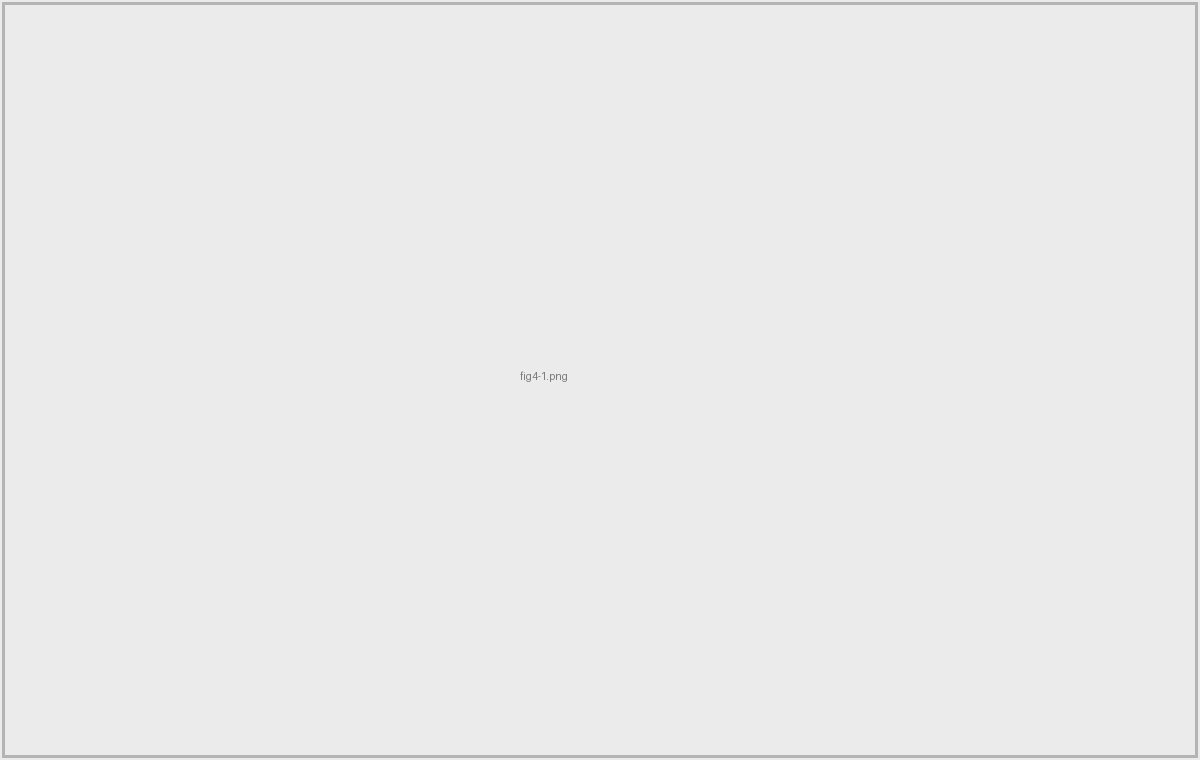
\includegraphics[width=\textwidth]{fig4-1.png}
    \caption{二维非笛卡尔成像的采样模式：二维回波平面（左上）、PROPELLER（右上）、径向（左下）与螺旋（右下）成像均涉及k空间至少在某一维上的非等距采样。}
    \label{fig:4.1}
\end{figure}

尽管如此，过去几十年中人们设计并探索了相当多样的、刻意不在笛卡尔网格上采集数据的方法。这些方法在二维情形下最流行的四种采样模式（包括投影重建，即径向成像）如图\autoref{fig:4.1}所示。

回波平面成像（Echo-Planar Imaging，EPI）\label{term:EPI}通常甚至不被视为一种非笛卡尔成像方法。它采用的梯度波形由一列极性交替的梯形脉冲构成，位于频率编码方向。图\autoref{fig:4.2}上方给出了这样一列波形的起始部分，其中$G$与$t$均已归一化。在其最纯粹的形式中，整个k空间在单次激励后沿方向相反的平行线被遍历。为进一步提高速度与效率，每条线上最初的若干样本在磁场梯度仍在爬升时就已经采集，最后若干样本在磁场梯度已经开始下降时仍在采集。这种所谓的斜坡采样导致频率编码方向上k空间边缘处的采样密度增大，而其他各处保持恒定的采样密度。数据采集仅在通过施加相位编码方向的磁场梯度来切换平行线时中断，并且在通过各方向上的第一个梯形脉冲到达k空间的一个角之前不会开始。EPI如今被广泛使用，尤其在扩散加权成像（Diffusion-Weighted Imaging，DWI）\label{term:DWI}与功能成像（functional MRI，fMRI）\label{term:fMRI}中。

\begin{figure}[ht]
    \centering
    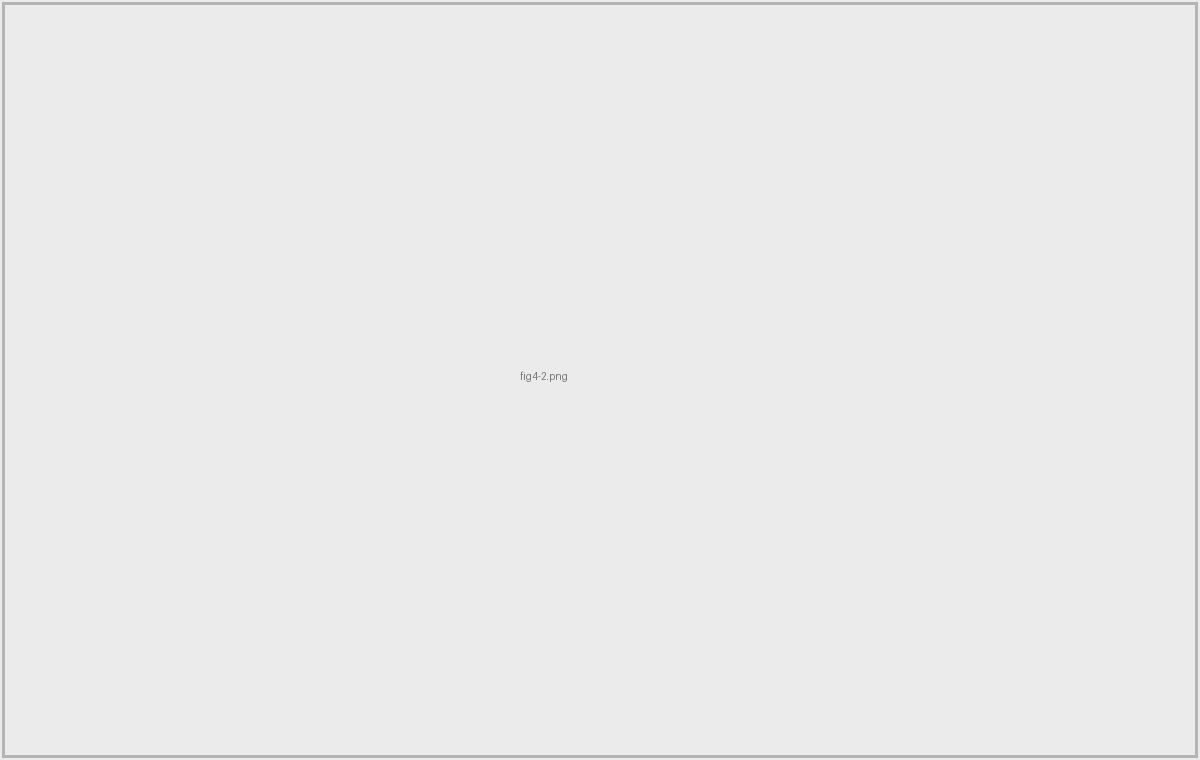
\includegraphics[width=\textwidth]{fig4-2.png}
    \caption{二维非笛卡尔成像的梯度波形：二维回波平面（上）、PROPELLER或径向（中）与螺旋（下）成像在频率编码与相位编码方向上依赖不同的梯度波形（原图为红色与绿色）以及不同的采集窗口（原图为蓝色），以产生\autoref{fig:4.1}中的采样模式。为简单起见，均假设基于梯度回波。}
    \label{fig:4.2}
\end{figure}

周期性旋转重叠平行线增强重建（Periodically Rotated Overlapping Parallel Lines with Enhanced Reconstruction，PROPELLER）\label{term:PROPELLER}成像也是一种笛卡尔与非笛卡尔的混合成像方法。其数据采集被分割为若干叶片，每个叶片覆盖一个矩形k空间区域。每个叶片支持基于逆FFT重建出一幅具有各向异性空间分辨率的中间图像。这些中间图像使得检测与校正各叶片采集之间的运动成为可能，其中各叶片之间围绕k空间原点相对旋转。然而，最终图像的重建必须应对所有叶片合起来造成的高度非均匀k空间采样。其梯度波形与笛卡尔成像相同，只是频率编码与相位编码方向随叶片一起旋转。PROPELLER成像在易受运动影响的应用中尤为重要，包括头部、颈部、脊柱与肩部成像。

径向成像主要用于那些k空间中心与边缘之间采样密度的剧烈变化确实能带来优势的领域。首先，中心的过采样通过对数据的不一致性进行大范围平均，带来对运动的不敏感性。此外，残余伪影在二维中扩散并表现为条纹，通常比笛卡尔成像中沿一维出现的相干或非相干鬼影更为温和（后者不存在采样密度的变化）。另外，对中心的重复覆盖使得动态成像中多种空间与时间分辨率的图像重建成为可能，也使得腹部与心脏成像在自由呼吸下无需插入导航回波或专用传感器即可实现回顾性自门控。此外，径向成像允许从中心开始数据采集从而省去相位编码，实现很短的回波时间以捕获快速衰减的信号，这在肺部与骨骼成像中是必需的。与PROPELLER成像相比，径向成像去掉了相位编码方向的梯度波形，而频率编码方向的梯度波形随投影一起旋转。频率编码方向上的第一个梯形脉冲被保留以获得完整投影，或被去除以获得半投影，这将在后面的实例中展示。

螺旋成像首先提供了快速而灵活的k空间覆盖。它支持单次激发与多次激发成像、除k空间最中心外处处均匀的采样密度、以及跨k空间的可变采样密度，还支持从中心向外和从边缘向内遍历k空间。与EPI不同，其磁场梯度在数据采集期间连续变化，消除了用于切换极性的死时间。此外，运动伪影与混叠伪影相当不相干，尤其是流动伪影不那么明显。螺旋成像主要受到要求高速度与高效率的广泛应用关注，但它对不理想的主磁场或磁场梯度非常敏感。

上述所有二维方法都可以扩展到三维，或者通过所谓的堆叠（在第三维上增加等距采样），或者通过适当的推广。

由于MRI中采样模式的多样性，非笛卡尔成像的重建更倾向于使用通用算法。考虑到MRI所能达到的信噪比（Signal-to-Noise Ratio，SNR）\label{term:SNR}有限，这类算法的精度只需达到中等即可，尤其与CT相比。这类算法的一个核心组成部分——非均匀快速Fourier变换（Nonequispaced Fast Fourier Transform，NFFT）\label{term:NFFT}——将在下一节介绍。在此基础上，再下一节将介绍普遍使用的网格化方法\footnote{生成k空间轨迹的梯度波形、以及由\autoref{equ:4.1}给出采样位置的推导，见第一章。}。

\section{非均匀快速Fourier变换（NFFT）}
如第二章所述，k空间中测得的信号$s$建模为
\begin{equation}
    s(\bm{k})=\int_{-N/2}^{N/2}x(\bm{r})\,\mathrm{e}^{-i2\pi\bm{k}\bm{r}}\,\mathrm{d}\bm{r},
    \label{equ:4.2}
\end{equation}
其中$x$表示最大范围为$[-N/2,N/2)$的物体的横向磁化强度，以下简称为物体与视野（Field of View，FOV）\label{term:FOV}。长度为$N$的FFT可以高效地将$x$的$N$个等距样本转换为由下式定义的$\tilde{s}$的$N$个等距样本
\begin{equation}
    \tilde{s}_m=\sum_{n=1}^{N}x_n\,\mathrm{e}^{-i2\pi k_m r_n}.
    \label{equ:4.3}
\end{equation}
这里$r$与$k$无量纲，分别归一化到$[-N/2,N/2)$与$[-1/2,1/2)$的范围。假设$N$为偶正整数，空间中的采样位置位于$r_n=-N/2,-N/2+1,\ldots,N/2-1$。由于采集对k空间的覆盖有限、以及重建中物体的空间离散化，$\tilde{s}$与$s$由下式相联系
\begin{equation}
    \tilde{s}(k)=\sum_{p=-\infty}^{\infty}s(k+p),
    \label{equ:4.4}
\end{equation}
因此\autoref{equ:4.3}中的$\tilde{s}_m$并不是$s$的样本，而是$s$变成周期为$1$的周期信号$\tilde{s}$后的样本。为把计算复杂度从直接求值\autoref{equ:4.3}的$O(N^2)$降到$O(N\log N)$，FFT利用了指数因子中的对称性；而当$r_n$或$k_m$不再等距时，这种对称性就丧失了。

NFFT将FFT推广到$x$、$\tilde{s}$或两者的非等距样本\footnote{指数因子的对称性指$\mathrm{e}^{-i2\pi k(r+1)}=\mathrm{e}^{-i2\pi kr}$的周期性、以及$\mathrm{e}^{-i2\pi(k+N/2)r}$与$\mathrm{e}^{i2\pi(k-N/2)r}$之间的共轭对称性等，这些性质使FFT可以按蝶形结构分解计算，从而把复杂度降到$O(N\log N)$。}。它依赖FFT完成空间域与空间频率域之间的实际变换，因此必须在中途把非等距样本转换为等距样本。这涉及一种近似，其精度可以与计算复杂度相权衡。以下考虑$x$为等距样本、$\tilde{s}$为非等距样本的情形。它与\autoref{equ:4.3}即正演模型的高效求值有关——在非笛卡尔成像中，正演模型需要从$N$个$x$的样本计算出$M$个$\tilde{s}$的样本。另外两种情形将在本章末尾讨论。

为把k空间中的等距样本转换为非等距样本，需要进行一次与窗函数$c$的卷积，$c$通过下式变成周期为$1$的周期函数$\tilde{c}$
\begin{equation}
    \tilde{c}(k)=\sum_{p=-\infty}^{\infty}c(k+p),
    \label{equ:4.5}
\end{equation}
假设$\tilde{c}$具有一致收敛的Fourier级数，从而可以写成
\begin{equation}
    \tilde{c}(k)=\sum_{r=-\infty}^{\infty}\tilde{c}_r\,\mathrm{e}^{i2\pi kr},
    \label{equ:4.6}
\end{equation}
其Fourier系数为
\begin{equation}
    \tilde{c}_r=\int_{-1/2}^{1/2}\tilde{c}(k)\,\mathrm{e}^{-i2\pi kr}\,\mathrm{d}k.
    \label{equ:4.7}
\end{equation}
将$k$替换为$k-k'$得到
\begin{equation}
    \tilde{c}_r=\int_{-1/2}^{1/2}\tilde{c}(k-k')\,\mathrm{e}^{-i2\pi(k-k')r}\,\mathrm{d}k',
    \label{equ:4.8}
\end{equation}
它可由下式近似
\begin{equation}
    \tilde{c}_r\approx\frac{1}{fN}\sum_{n'=-fN/2}^{fN/2-1}\tilde{c}\left(k-\frac{n'}{fN}\right)\mathrm{e}^{-i2\pi\left(k-\frac{n'}{fN}\right)r}.
    \label{equ:4.9}
\end{equation}
引入过采样因子$f\ge 1$以提高精度，其中$fN$也假设为偶正整数。若周期函数$\tilde{c}$是带限的、最高频率为$fN/2$，则\autoref{equ:4.9}精确成立。否则会出现混叠，$\tilde{c}_r$的估计会受到更高频率的干扰。更具体地说，对任意非零整数$p$，频带$[fNp-N/2,fNp+N/2)$会折叠回基带$[-N/2,N/2)$。整理\autoref{equ:4.9}可得
\begin{equation}
    \mathrm{e}^{i2\pi kr}\approx\frac{1}{fN\tilde{c}_r}\sum_{n'=-fN/2}^{fN/2-1}\tilde{c}\left(k-\frac{n'}{fN}\right)\mathrm{e}^{i2\pi\frac{n'}{fN}r},
    \label{equ:4.10}
\end{equation}
前提是$\tilde{c}_r\neq 0$；再将$r$替换为$-r$得到
\begin{equation}
    \mathrm{e}^{-i2\pi kr}\approx\frac{1}{fN\tilde{c}_{-r}}\sum_{n'=-fN/2}^{fN/2-1}\tilde{c}\left(k-\frac{n'}{fN}\right)\mathrm{e}^{-i2\pi\frac{n'}{fN}r},
    \label{equ:4.11}
\end{equation}
将其代入\autoref{equ:4.3}得到
\begin{equation}
    \tilde{s}_m\approx\sum_{n'=-fN/2}^{fN/2-1}\tilde{c}\left(\frac{k_m-n'}{fN}\right)\sum_{n=1}^{N}\frac{x_n}{fN\tilde{c}_{-r_n}}\mathrm{e}^{-i2\pi\frac{n'}{fN}r_n}.
    \label{equ:4.12}
\end{equation}
内层求和相当于一次长度为$fN$的FFT：它把空间中的$N$个等距的$x$样本（加权并补零到$fN$个空间的样本后）变换为k空间中的$fN$个等距样本。外层求和则通过一次卷积把后者转换为k空间中的$M$个非等距样本。

选择
\begin{equation}
    \tilde{c}_r=\begin{cases}
        \dfrac{1}{fN}, & -\dfrac{fN}{2}<r\le\dfrac{fN}{2}\\[2mm]
        0, & \text{其他}
    \end{cases}
    \label{equ:4.13}
\end{equation}
可以省去加权（通常称为去变迹，deapodization），并由\autoref{equ:4.6}得到
\begin{equation}
    \tilde{c}(k)=\frac{1}{fN}\sum_{r=-fN/2+1}^{fN/2}\mathrm{e}^{i2\pi kr}.
    \label{equ:4.14}
\end{equation}
这里$r$取值范围的变化来自\autoref{equ:4.11}中把$r$替换为$-r$。此时$\tilde{c}(k)$是一个次数为$fN/2$的复三角多项式，对它可以精确成立\autoref{equ:4.9}。它可写为
\begin{equation}
    \tilde{c}(k)=\begin{cases}
        \dfrac{\sin(\pi kfN)}{fN\sin(\pi k)}\mathrm{e}^{i\pi k}, & k\neq 0\\[2mm]
        1, & \text{其他}
    \end{cases}
    \label{equ:4.15}
\end{equation}
并在$\pi k$较小时用
\begin{equation}
    \tilde{c}(k)\approx\operatorname{sinc}(\pi kfN)
    \label{equ:4.16}
\end{equation}
近似，其中
\begin{equation}
    \operatorname{sinc}(x)=\begin{cases}
        \dfrac{\sin(x)}{x}, & x\neq 0\\[2mm]
        1, & \text{其他}
    \end{cases}
    \label{equ:4.17}
\end{equation}
根据采样定理，$s$可由其等距样本恢复
\begin{equation}
    s(k)=\sum_{n=-\infty}^{\infty}s\left(\frac{n}{fN}\right)\operatorname{sinc}\left(\pi\left(k-\frac{n}{fN}\right)fN\right).
    \label{equ:4.18}
\end{equation}
因此，在采集对k空间的覆盖不受限这一假想情形下，无限支撑的sinc函数就是理想的窗函数。然而在覆盖受限的实际情形下，根据\autoref{equ:4.15}，更好的做法是用周期化后的sinc函数来替代它，并乘上由偶数$fN$时$r_n$的不对称性产生的相位因子$\mathrm{e}^{i\pi k}$——这就是所谓的Dirichlet核\footnote{Dirichlet核：形如$D_N(x)=\sum_{k=-N}^{N}\mathrm{e}^{ikx}$的三角多项式，其闭式解为$\sin((N+1/2)x)/\sin(x/2)$，是周期函数Fourier级数部分和的核心。此处\autoref{equ:4.15}即周期化sinc函数的Dirichlet核形式。}。

为降低卷积的计算复杂度，窗函数最好取实值、且其支撑有限，无论通过设计还是通过截断，都限制在$[-K/(2fN),K/(2fN)]$内，其中正整数$K$称为核尺寸。截断给出
\begin{equation}
    c'(k)=\begin{cases}
        c(k), & |k|\le\dfrac{K}{2fN}\\[2mm]
        0, & \text{其他}
    \end{cases}
    \label{equ:4.19}
\end{equation}
以及相应的周期为$1$的周期函数$\tilde{c}'$，并把\autoref{equ:4.12}变为
\begin{equation}
    \tilde{s}_m\approx\sum_{n'=-fN/2}^{fN/2-1}\tilde{c}'\left(\frac{k_m-n'}{fN}\right)\sum_{n=1}^{N}\frac{x_n}{fN\tilde{c}_{-r_n}}\mathrm{e}^{-i2\pi\frac{n'}{fN}r_n}.
    \label{equ:4.20}
\end{equation}

长椭球波函数能使一个给定支撑的函数在一个域中的相对能量、在另一个域的给定区间内达到最大。连续情形下，Kaiser--Bessel窗是它们的一个简单近似。因此它特别适合用来最小化\autoref{equ:4.12}中的混叠误差与\autoref{equ:4.20}中的截断误差。若以最小化混叠误差为目标，去变迹由Kaiser--Bessel窗定义为
\begin{equation}
    \tilde{c}_r=\begin{cases}
        \dfrac{1}{fNI_0(b)}I_0\left(b\sqrt{1-\left(\dfrac{\pi K}{fNb}r\right)^2}\right), & |r|\le\dfrac{fNb}{\pi K}\\[3mm]
        0, & \text{其他}
    \end{cases},
    \label{equ:4.21}
\end{equation}
其中$I_0$是第一类零阶修正Bessel函数。把形状参数$b$取为
\begin{equation}
    b=\pi K\left(1-\frac{1}{2f}\right),
    \label{equ:4.22}
\end{equation}
可使Fourier系数在$|r|>fN-\frac{N}{2}$时降为零。此时窗函数（也称为卷积核）由下式给出
\begin{equation}
    c(k)=\begin{cases}
        \dfrac{2b}{\pi K}\operatorname{sinhc}\left(b\sqrt{1-\left(\dfrac{2fN}{K}k\right)^2}\right), & |k|\le\dfrac{K}{2fN}\\[3mm]
        \dfrac{2b}{\pi K}\operatorname{sinc}\left(b\sqrt{\left(\dfrac{2fN}{K}k\right)^2-1}\right), & \text{其他}
    \end{cases}
    \label{equ:4.23}
\end{equation}
其中用到
\begin{equation}
    \operatorname{sinhc}(x)=\begin{cases}
        \dfrac{\sinh(x)}{x}, & x\neq 0\\[2mm]
        1, & \text{其他}
    \end{cases}.
    \label{equ:4.24}
\end{equation}
若转而以最小化截断误差为目标，则卷积核由Kaiser--Bessel窗定义为
\begin{equation}
    c(k)=\begin{cases}
        \dfrac{1}{KI_0(b)}I_0\left(b\sqrt{1-\left(\dfrac{2fN}{K}k\right)^2}\right), & |k|\le\dfrac{K}{2fN}\\[3mm]
        0, & \text{其他}
    \end{cases},
    \label{equ:4.25}
\end{equation}
而去变迹由下式给出
\begin{equation}
    \tilde{c}_r=\begin{cases}
        \dfrac{1}{fN}\operatorname{sinhc}\left(b\sqrt{1-\left(\dfrac{\pi K}{fNb}r\right)^2}\right), & |r|\le\dfrac{fNb}{\pi K}\\[3mm]
        \dfrac{1}{fN}\operatorname{sinc}\left(b\sqrt{\left(\dfrac{\pi K}{fNb}r\right)^2-1}\right), & \text{其他}
    \end{cases}.
    \label{equ:4.26}
\end{equation}
两种选择导致相似的卷积核与去变迹，如图\autoref{fig:4.3}与\autoref{fig:4.4}所示，其中$f=2.0$、$K=5$、$N=800$，函数值被归一化到$[0,1]$范围。

值得注意的是，\autoref{equ:4.23}与\autoref{equ:4.26}中的第二种情形只是为了完整性而给出。由于卷积核被截断、且物体支撑有限，实际中只有第一种情形是相关的。此外，从\autoref{equ:4.21}与\autoref{equ:4.25}的第一种情形中分别减去偏移$\frac{1}{fNI_0(b)}$与$\frac{1}{KI_0(b)}$，可使Kaiser--Bessel窗在$|r|=\frac{fNb}{\pi K}$与$|k|=\frac{K}{2fN}$处就已平滑地降为零，从而分别能够消除混叠误差、并防止卷积核在最坏情况下延伸到k空间中$K+1$个等距样本之外。

\begin{figure}[ht]
    \centering
    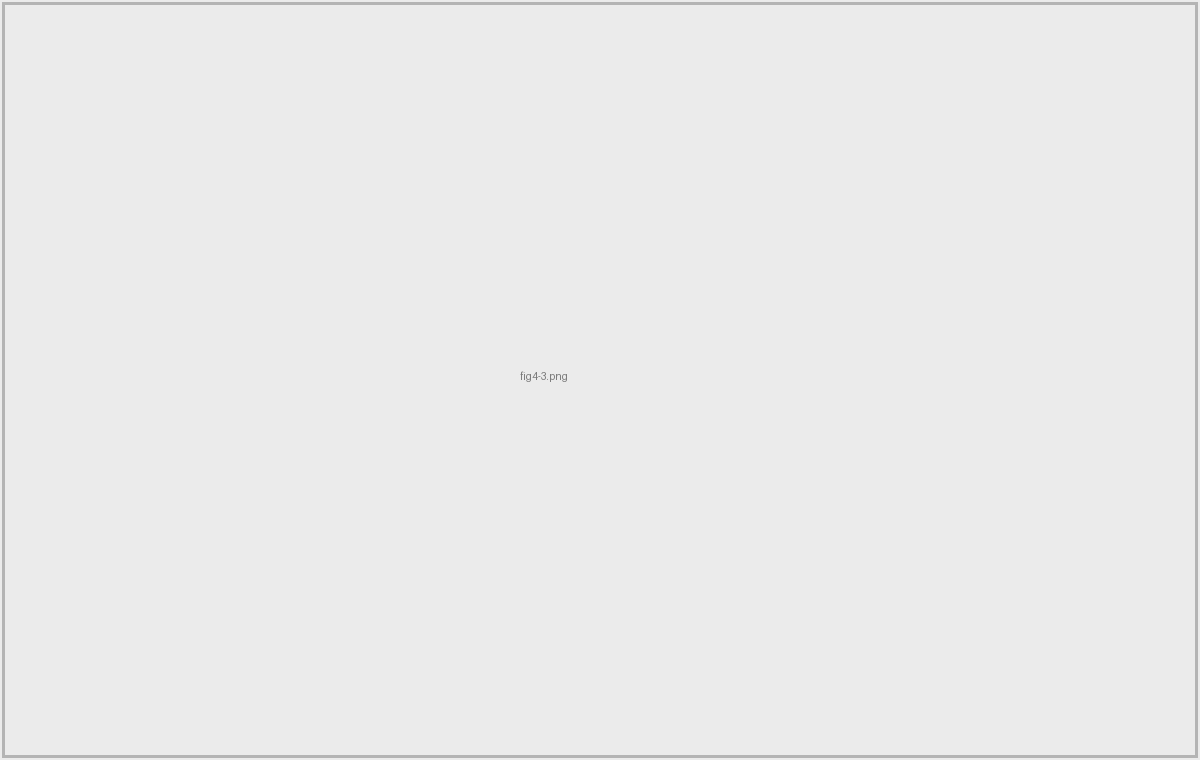
\includegraphics[width=\textwidth]{fig4-3.png}
    \caption{卷积核与去变迹：在k空间中等距样本向非等距样本的转换中，采用Kaiser--Bessel窗的Fourier变换作为卷积核（左，原图为红色实线），为补偿固有的低通滤波，在空间中除以Kaiser--Bessel窗进行去变迹（右，原图为红色实线）；另一种方案是以Kaiser--Bessel窗作为卷积核（左，原图为绿色虚线），并除以Kaiser--Bessel窗的逆Fourier变换作为去变迹（右，原图为绿色虚线）。}
    \label{fig:4.3}
\end{figure}

\begin{figure}[ht]
    \centering
    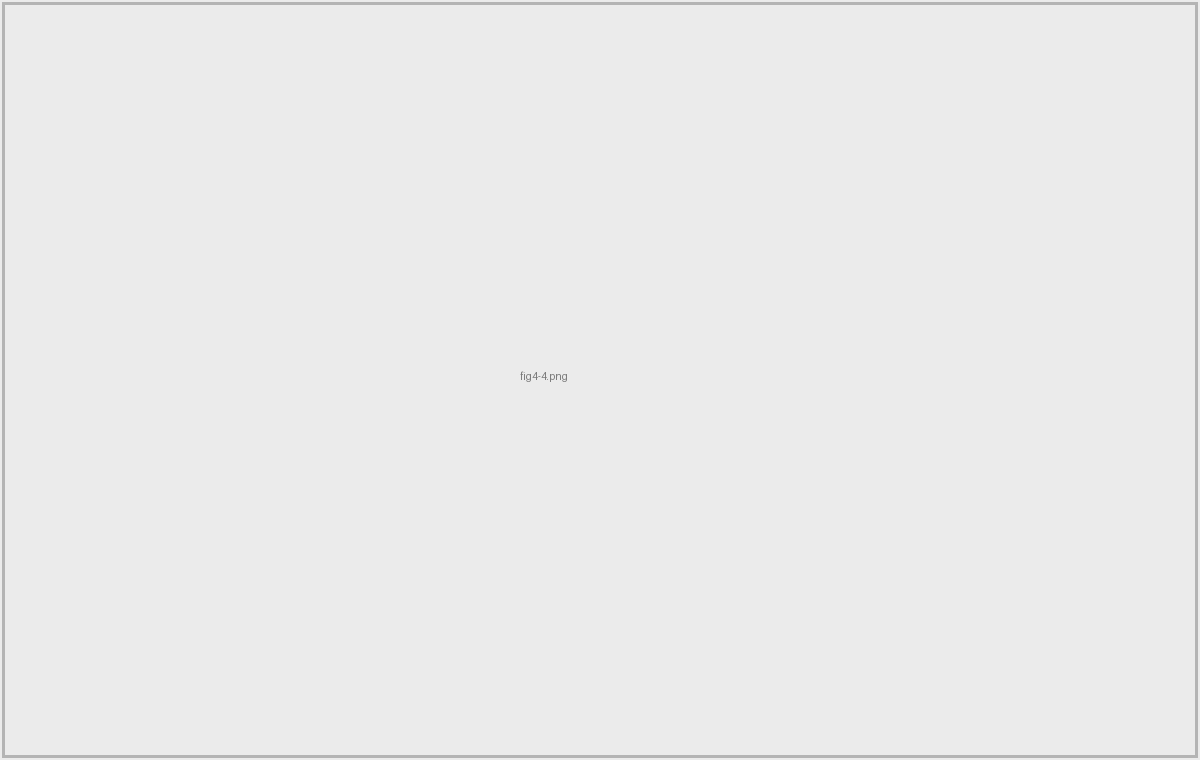
\includegraphics[width=\textwidth]{fig4-4.png}
    \caption{混叠误差与截断误差：\autoref{fig:4.3}中的卷积核及其逆Fourier变换在更大范围的$k$与$r$上以对数刻度显示。Kaiser--Bessel窗是具有紧支撑的函数，其Fourier变换与逆Fourier变换却不是。因此，在空间中使用Kaiser--Bessel窗作去变迹会在k空间中产生截断误差（原图为红色实线），而将其用作k空间中的卷积核则会在空间中产生混叠误差（原图为绿色虚线）。图中还标出了规定的核尺寸与FOV（左、右原图为黑色实线）、过采样扩展后的FOV（右，原图为黑色虚线）以及折叠回规定FOV的前三个频带（右，原图为蓝色实线、虚线与点线）。}
    \label{fig:4.4}
\end{figure}

一般而言，NFFT的精度与计算复杂度都随过采样因子与核尺寸增大而增大。针对各种窗函数已经建立了误差界，用以在给定目标精度下指导$f$与$K$最小取值的选取。由于FFT的运行时间并不随FFT长度单调增长，$f$的选取最好参照长度为$fN$的FFT的运行时间。窗函数的复杂度则不那么重要，因为它通常只计算一次并存储在查找表中。

\autoref{equ:4.20}可改写为
\begin{equation}
    \tilde{\bm{s}}\approx\mathbf{C}'\mathbf{F}\mathbf{D}\bm{x},
    \label{equ:4.27}
\end{equation}
其中$\mathbf{D}$为$N\times N$的对角去变迹矩阵
\begin{equation}
    [\mathbf{D}]_{n,n}=\frac{1}{fN\tilde{c}_{-r_n}},
    \label{equ:4.28}
\end{equation}
$\mathbf{F}$为$fN\times N$的Fourier变换矩阵
\begin{equation}
    [\mathbf{F}]_{n',n}=\mathrm{e}^{-i2\pi\left(\frac{n'-1}{fN}-\frac{1}{2}\right)r_n},
    \label{equ:4.29}
\end{equation}
$\mathbf{C}'$为稀疏的$M\times fN$卷积矩阵
\begin{equation}
    [\mathbf{C}']_{m,n'}=\tilde{c}'\left(k_m-\frac{n'-1}{fN}+\frac{1}{2}\right).
    \label{equ:4.30}
\end{equation}
这里矩阵的列与行从1开始编号，这使得\autoref{equ:4.29}与\autoref{equ:4.30}括号内的表达式比\autoref{equ:4.20}更复杂\footnote{若把\autoref{equ:4.20}中从$-fN/2$到$fN/2-1$的求和指标换成从1到$fN$（即$n'_{\text{new}}=n'+fN/2+1$），则\autoref{equ:4.29}与\autoref{equ:4.30}中的$\frac{n'-1}{fN}-\frac{1}{2}$恰与$\frac{n'}{fN}$一致。}。\autoref{equ:4.27}是下式的近似
\begin{equation}
    \tilde{\bm{s}}=\mathbf{E}\bm{x}
    \label{equ:4.31}
\end{equation}
其中$\mathbf{E}$为$M\times N$的编码矩阵
\begin{equation}
    [\mathbf{E}]_{m,n}=\mathrm{e}^{-i2\pi k_mr_n}.
    \label{equ:4.32}
\end{equation}
本章始终假设$M$与$N$量级相同，暂不考虑Fourier插值。欠采样是后续各章的主题。

把NFFT扩展到多维可以通过张量积方法直接完成。可分离卷积核（由各维一维卷积核的乘积定义）使用方便且在实际中占主导地位，而不可分离卷积核（如圆对称与球对称核）则有望在给定的目标计算复杂度下提高精度。然而，对二者的理论比较似乎仍然缺失。

\section{网格化}
物体$\bm{x}$理想上可由信号$s$恢复
\begin{equation}
    x(\bm{r})=\int_{-\infty}^{\infty}s(\bm{k})\,\mathrm{e}^{i2\pi\bm{k}\bm{r}}\,\mathrm{d}\bm{k}.
    \label{equ:4.33}
\end{equation}
由于采集对k空间的覆盖有限，$s$只在$\bm{k}\in[-1/2,1/2)$上已知，在其他地方若无先验知识则被忽略，这导致近似
\begin{equation}
    \hat{x}(\bm{r})=\int_{-1/2}^{1/2}s(\bm{k})\,\mathrm{e}^{i2\pi\bm{k}\bm{r}}\,\mathrm{d}\bm{k}.
    \label{equ:4.34}
\end{equation}
此外，$s$是以有限分辨率采样的：在频率编码方向上受硬件约束限制，在相位编码方向上更根本地受时间约束限制，从而得到进一步的近似
\begin{equation}
    \hat{x}_n=\frac{1}{M}\sum_{m=1}^{M}s_m\,\mathrm{e}^{i2\pi k_mr_n}
    \label{equ:4.35}
\end{equation}
或
\begin{equation}
    \hat{\bm{x}}=\frac{1}{M}\mathbf{E}^H\bm{s}.
    \label{equ:4.36}
\end{equation}
长度为$M$的逆FFT可以高效地把$s$的$M$个等距样本转换为$\hat{\bm{x}}$的$M$个等距样本。若要以更高的空间分辨率重建物体，即通过Fourier插值将其放大，这里把$\hat{\bm{x}}$的等距样本数、从而把逆FFT的长度增加到$N>M$，同时把$s$的等距样本间距减小到$\frac{1}{N}$。与\autoref{equ:4.14}和\autoref{equ:4.15}类似，把$x$与$\hat{x}$联系起来的点扩散函数（Point Spread Function，PSF）\label{term:PSF}此时为
\begin{equation}
    \begin{aligned}
        \operatorname{PSF}(r)&=\frac{1}{M}\sum_{m=-M/2}^{M/2-1}\mathrm{e}^{i2\pi\frac{m}{N}r}\\
        &=\frac{\sin\left(\pi\frac{r}{N}M\right)}{M\sin\left(\pi\frac{r}{N}\right)}\mathrm{e}^{-i\pi\frac{r}{N}},
    \end{aligned}
    \label{equ:4.37}
\end{equation}
其中缩放的选取使得$\operatorname{PSF}(0)=1$。因此，$\hat{\bm{x}}$的等距样本之间近似由sinc插值相联系。只有在$N=M$这种例外情形下（因为临床常规中几乎总是应用Fourier插值），它们才是不相关的。

逆FFT既是相应FFT的伴随、又是其逆。对NFFT而言这不再成立。网格化最初是在射电天文学中由更简单的插值方法发展而来，并在NFFT被提出并在数学上得到透彻分析之前就被医学成像采用。它的目标是从$s$的$M$个非等距样本重建$x$的$N$个等距样本。

为提供NFFT的近似显式逆，网格化依赖于一次伴随NFFT，并引入对$s$的非等距样本的额外加权，即采样密度补偿（sampling density compensation）。它描述为
\begin{equation}
    \hat{\bm{x}}\approx\mathbf{D}^H\mathbf{F}^H\mathbf{C}'^H\mathbf{W}\bm{s},
    \label{equ:4.38}
\end{equation}
其中$\mathbf{W}$是由权向量$\bm{w}$构成的对角矩阵$M\times M$。因此，在采样密度补偿之后，它涉及一次与窗函数的卷积、一次逆FFT以及一次去变迹。与上一节推导的NFFT相比，这三个步骤以相反的顺序执行。此外，卷积在过采样的笛卡尔网格上求值，FFT被替换为逆FFT，扩展后的FOV被去变迹裁剪掉\footnote{这里的“逆”是相对的：NFFT把空间等距样本转换为k空间非等距样本；网格化则先把k空间非等距样本加权，再经卷积、逆FFT与去变迹回到空间等距样本。三步骤取相反顺序，是因为每一步的算子都需取伴随或逆。}。

人们提出了各种导出合适采样密度补偿的方法。一类方法把每个$s_m$视为k空间中某个邻域的代表，并把\autoref{equ:4.35}变为Riemann和
\begin{equation}
    \hat{x}_n=\sum_{m=1}^{M}w_ms_m\,\mathrm{e}^{i2\pi k_mr_n}.
    \label{equ:4.39}
\end{equation}
这里，对应于某一维长度的正权之和被归一化为$1$。权的计算基于连续模型或离散模型。

对简单的非笛卡尔采样模式，权可以由可微坐标变换的Jacobi行列式解析地得到。在二维径向成像中，从极坐标网格到笛卡尔网格的坐标变换定义为
\begin{equation}
    k_x=k_r\cos(2\pi k_\phi)\qquad k_y=k_r\sin(2\pi k_\phi),
    \label{equ:4.40}
\end{equation}
其中径向方向$k_r$与方位角方向$k_\phi$分别归一化到$[0,\frac{1}{2}]$与$[-\frac{1}{2},\frac{1}{2})$。Jacobi矩阵
\begin{equation}
    \mathbf{J}_R=\begin{bmatrix}
        \dfrac{\partial k_x}{\partial k_r} & \dfrac{\partial k_x}{\partial k_\phi}\\[3mm]
        \dfrac{\partial k_y}{\partial k_r} & \dfrac{\partial k_y}{\partial k_\phi}
    \end{bmatrix}
    \label{equ:4.41}
\end{equation}
的行列式等于$2\pi k_r$。把\autoref{equ:4.34}中的积分扩展到二维中半径为$\frac{1}{2}$的圆形区域$R$，得到
\begin{equation}
    \hat{x}(r_x,r_y)=\iint_{R}s(k_x,k_y)\,\mathrm{e}^{i2\pi(k_xr_x+k_yr_y)}\,\mathrm{d}k_x\,\mathrm{d}k_y
    \label{equ:4.42}
\end{equation}
以及变量替换后的
\begin{equation}
    \hat{x}(r_x,r_y)=2\pi\int_{0}^{1/2}\int_{-1/2}^{1/2}s(k_r,k_\phi)k_r\,\mathrm{e}^{i2\pi k_r\left(\cos(2\pi k_\phi)r_x+\sin(2\pi k_\phi)r_y\right)}\,\mathrm{d}k_\phi\,\mathrm{d}k_r.
    \label{equ:4.43}
\end{equation}
相应地，$s(k_r,k_\phi)$被$2\pi k_r$加权，这对应于反投影中使用的理想斜坡滤波器。

在二维螺旋成像中，对一些常见的k空间轨迹存在到极坐标网格的坐标变换，并且可以方便地推广为到笛卡尔网格的坐标变换。对于分段（或称交错）的可变角速度k空间轨迹，如图\autoref{fig:4.1}右下所示，它定义为
\begin{equation}
    \begin{aligned}
        k_r&=\frac{k_s}{2\sqrt{\alpha}+(1-\alpha)k_s}\\
        k_\phi&=\frac{N}{M_I}\cdot\frac{k_s}{2\sqrt{\alpha}+(1-\alpha)k_s}+k_i,
    \end{aligned}
    \label{equ:4.44}
\end{equation}
其中$k_s$参数化一条交错线上的样本（即时间），归一化到$[0,1]$；$k_i$参数化交错线（即它绕k空间原点的旋转），归一化到$[-\frac{1}{2},\frac{1}{2})$。这里$k_s$与$k_i$都被视为连续的。$k_\phi$的范围扩展到$[-\frac{1}{2},\frac{1}{2}+\frac{N}{2M_I})$，而$M$被细分为$M_I$条交错线、每条$M_S$个样本。由于
\begin{equation}
    k_r=\frac{M_I}{N}(k_\phi-k_i),
    \label{equ:4.45}
\end{equation}
这是一个参数$\alpha\in[0,1]$的Archimedes螺线。$\alpha=0$与$\alpha=1$分别对应恒定线速度螺旋与恒定角速度螺旋。Jacobi矩阵
\begin{equation}
    \mathbf{J}_S=\begin{bmatrix}
        \dfrac{\partial k_r}{\partial k_s} & \dfrac{\partial k_r}{\partial k_i}\\[3mm]
        \dfrac{\partial k_\phi}{\partial k_s} & \dfrac{\partial k_\phi}{\partial k_i}
    \end{bmatrix}
    \label{equ:4.46}
\end{equation}
的行列式由下式给出
\begin{equation}
    |\mathbf{J}_S|=\frac{2\alpha+(1-\alpha)k_s}{4\left(\alpha+(1-\alpha)k_s\right)^{\frac{3}{2}}},
    \label{equ:4.47}
\end{equation}
而到笛卡尔网格的复合坐标变换的Jacobi行列式为
\begin{equation}
    |\mathbf{J}_S\mathbf{J}_R|=\frac{\pi}{4}\cdot\frac{2\alpha k_s+(1-\alpha)k_s^2}{\left(\alpha+(1-\alpha)k_s\right)^2}.
    \label{equ:4.48}
\end{equation}
对于更复杂的非笛卡尔采样模式，权可以通过构造Voronoi图并计算每个Voronoi单元的面积，从离散的k空间采样位置几何地得到\footnote{Voronoi图：给定平面上的一组点，每个点对应一个Voronoi单元，单元内任意位置到该点的距离都小于到其他点的距离。因此，Voronoi单元的面积可作为该采样点在k空间中所代表区域的面积，即采样密度补偿的权。}。

另一类方法求解一个极小化问题。例如，把\autoref{equ:4.38}中的$\bm{s}$用\autoref{equ:4.27}的$\tilde{\bm{s}}$替换得到
\begin{equation}
    \hat{\bm{x}}\approx\mathbf{D}^H\mathbf{F}^H\mathbf{C}'^H\mathbf{W}\mathbf{C}'\mathbf{F}\mathbf{D}\bm{x}.
    \label{equ:4.49}
\end{equation}
与\autoref{equ:4.13}和\autoref{equ:4.14}类似，把稀疏卷积矩阵$\mathbf{C}'$变成稠密卷积矩阵$\mathbf{C}$，就可以通过令$\mathbf{D}=\mathbf{I}$来消去去变迹。再取$f=1.0$，则\autoref{equ:4.49}简化为
\begin{equation}
    \mathbf{F}\hat{\bm{x}}\approx N\,\mathbf{C}^H\mathbf{W}\mathbf{C}\mathbf{F}\bm{x}
    \label{equ:4.50}
\end{equation}
因为$\mathbf{F}\mathbf{F}^H=N\mathbf{I}$。理想情况下，把正演模型作用于一幅图像、然后网格化得到模拟信号，应当能恢复该图像。与$\bm{x}$无关地，这将由条件
\begin{equation}
    N\,\mathbf{C}^H\mathbf{W}\mathbf{C}=\mathbf{I}
    \label{equ:4.51}
\end{equation}
保证。然而，该矩阵方程通常是超定的。可以把\autoref{equ:4.51}改写为包含$N^2$个方程的线性方程组并在左端乘以系统矩阵，或者转而最小化矩阵$N\mathbf{C}^H\mathbf{W}\mathbf{C}-\mathbf{I}$的Frobenius范数。两种方法都导致同样的、含$M$个方程的线性系统
\begin{equation}
    \mathbf{A}\bm{w}=\bm{b}
    \label{equ:4.52}
\end{equation}
其中
\begin{equation}
    [\mathbf{A}]_{m,m'}=\left|\left[\mathbf{C}\mathbf{C}^H\right]_{m,m'}\right|^2\qquad [\bm{b}]_m=\frac{1}{N}\left[\mathbf{C}\mathbf{C}^H\right]_{m,m}.
    \label{equ:4.53}
\end{equation}
由于条件数通常很差、计算复杂度又高，求解\autoref{equ:4.52}只对样本数较少的非笛卡尔采样模式可行。值得注意的是，由最小二乘近似\autoref{equ:4.51}得到的权不再一定为正。

类似地，要求信号在k空间中（而非图像在空间中）的一致性，可导出
\begin{equation}
    N\,\mathbf{C}\mathbf{C}^H\mathbf{W}=\mathbf{I}.
    \label{equ:4.54}
\end{equation}
若只考虑左右两端所得矩阵的对角元来放松该条件，它退化为
\begin{equation}
    N\,\mathbf{C}\mathbf{C}^H\bm{w}=\bm{1}.
    \label{equ:4.55}
\end{equation}
为求解\autoref{equ:4.55}，有人提出了如下不动点迭代
\begin{equation}
    \left[\bm{w}^{[i+1]}\right]_m=\frac{\left[\bm{w}^{[i]}\right]_m}{N\left[\mathbf{C}\mathbf{C}^H\bm{w}^{[i]}\right]_m},
    \label{equ:4.56}
\end{equation}
在使用截断卷积核时，它对样本数更多的非笛卡尔采样模式仍然可行。

网格化的一种推广是用空间变化的卷积核替代采样密度补偿。它有望带来更好的精度，但需要针对每种采样模式优化一次卷积核。

\section{迭代重建}
本节主要作为后面实例中网格化的参照，基于NFFT与伴随NFFT推导非笛卡尔成像的迭代重建。把\autoref{equ:4.31}中的$\tilde{\bm{s}}$替换为$\bm{s}$，得到正演模型
\begin{equation}
    \bm{s}=\mathbf{E}\bm{x}.
    \label{equ:4.57}
\end{equation}
逆问题通过最小二乘近似求解
\begin{equation}
    \min_{\hat{\bm{x}}}\left\|\bm{s}-\mathbf{E}\hat{\bm{x}}\right\|_2^2
    \label{equ:4.58}
\end{equation}
使用第一类正规方程
\begin{equation}
    \mathbf{E}^H\mathbf{E}\hat{\bm{x}}=\mathbf{E}^H\bm{s}
    \label{equ:4.59}
\end{equation}
或通过加权最小二乘近似
\begin{equation}
    \min_{\hat{\bm{x}}}\sum_{m=1}^{M}[\bm{w}]_m\left|\left(\bm{s}-\mathbf{E}\hat{\bm{x}}\right)_m\right|^2
    \label{equ:4.60}
\end{equation}
使用第一类修正正规方程
\begin{equation}
    \mathbf{E}^H\mathbf{W}\mathbf{E}\hat{\bm{x}}=\mathbf{E}^H\mathbf{W}\bm{s}.
    \label{equ:4.61}
\end{equation}
这里假设\autoref{equ:4.57}是超定的。欠采样与多接收线圈将在后续各章考虑。此外，向量$\bm{w}$与对角矩阵$\mathbf{W}$正是\autoref{equ:4.38}中为采样密度补偿引入的那两个。

为确定\autoref{equ:4.59}或\autoref{equ:4.61}中的$\hat{\bm{x}}$，最好采用迭代方法，例如第三章介绍的共轭梯度（Conjugate Gradient，CG）\label{term:CG}法。它们通常涉及反复计算系统矩阵与向量$\hat{\bm{p}}$的乘积。这些乘积既可以用NFFT与伴随NFFT高效计算，也可以用快速卷积高效计算。对于后者，系统矩阵的元素写为
\begin{equation}
    \left[\mathbf{E}^H\mathbf{E}\right]_{n,n'}=\sum_{m=1}^{M}\mathrm{e}^{i2\pi k_m\left(r_n-r_{n'}\right)}
    \label{equ:4.62}
\end{equation}
或
\begin{equation}
    \left[\mathbf{E}^H\mathbf{W}\mathbf{E}\right]_{n,n'}=\sum_{m=1}^{M}w_m\mathrm{e}^{i2\pi k_m\left(r_n-r_{n'}\right)}
    \label{equ:4.63}
\end{equation}
并记作$q(r_n-r_{n'})$。值得注意的是，$q(r)$与使用伴随NFFT或网格化的重建的PSF非常对应。此时这些乘积化为空间中的卷积
\begin{equation}
    \sum_{n'=1}^{N}\hat{p}_{n'}q(r_n-r_{n'}),
    \label{equ:4.64}
\end{equation}
它可以通过k空间中的一次乘法来求值。这样，NFFT与伴随NFFT本质上被一次FFT与一次逆FFT取代。$q$的Fourier变换只需计算一次。为避免折叠回来，快速卷积需要两倍的过采样。尽管如此，当$M\ge N$时它通常能带来可观的加速。

迭代方法可以合成采集所覆盖的k空间区域之外的信号。这尤其关系到方形k空间的四个角——如果实际只采样了该正方形的内切圆。由于恢复这类信号是病态的，它通常会导致高频噪声的过度放大，如第二章所讨论的那样。通常对$\hat{\bm{x}}$施加低通滤波以避免这一点。

\section{实例}
本节用一个一维与一个二维实例来说明网格化。图\autoref{fig:4.5}所示的三角形函数作为一维实例中的物体。该物体的Fourier变换由下式给出
\begin{equation}
    s(k_x)=R\operatorname{sinc}^2(\pi Rk_x),
    \label{equ:4.65}
\end{equation}
其中$R=320$。

\begin{figure}[ht]
    \centering
    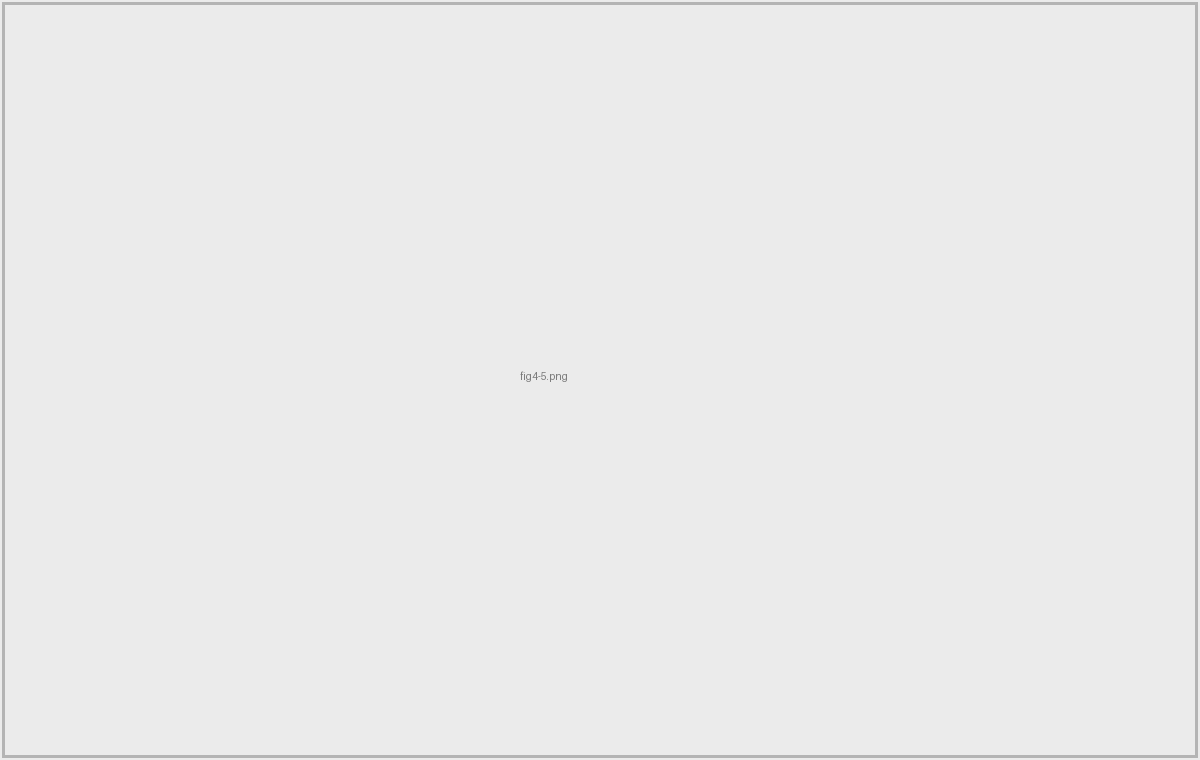
\includegraphics[width=\textwidth]{fig4-5.png}
    \caption{一维物体：选取一个连续三角形函数作为一维物体，其覆盖FOV的80\%（左）。其频谱为实值且非负（右）。}
    \label{fig:4.5}
\end{figure}

首先假设$s$以$k_x\in[-\frac{1}{4},\frac{1}{4})$、$M=400$等距采样。这允许用逆FFT作为参照，并评估网格化引入的混叠误差或截断误差。物体在$r_x=-\frac{N}{2},-\frac{N}{2}+1,\ldots,\frac{N}{2}-1$处以$N=800$重建。因此它被Fourier插值放大了$2$倍，涉及在k空间中补零到$[-\frac{1}{2},\frac{1}{2})$。所得误差绘制于图\autoref{fig:4.6}，主要由$r_x=-320,0,320$处的振铃伪影主导。三角形函数在这些点是连续的但不可微。因此并未观察到经典Gibbs现象，但由于Fourier系数随频率衰减更慢，预期会得到更差的截断Fourier级数近似。与逆FFT相比，取$f=2$与$K=5$的网格化只引入了可忽略的误差，来自此情形下卷积核的截断。以下保持过采样因子与核尺寸的这些设置。

\begin{figure}[ht]
    \centering
    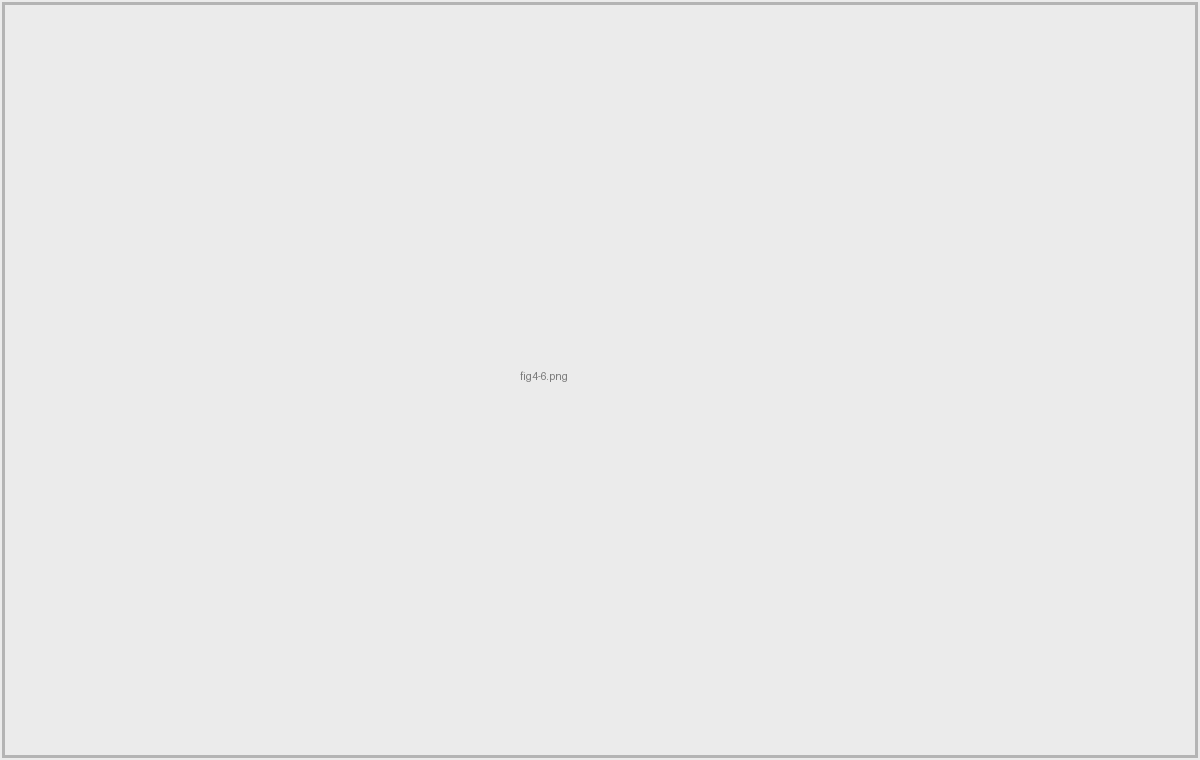
\includegraphics[width=\textwidth]{fig4-6.png}
    \caption{一维笛卡尔采样：逆FFT与网格化对比。由图\autoref{fig:4.5}中频谱$s$的等距采样，以两倍空间分辨率重建一维物体$\hat{x}$，分别使用逆FFT（左）与网格化（右），均涉及补零。误差相对于连续三角形函数$x$计算。}
    \label{fig:4.6}
\end{figure}

为模拟$s$的非等距采样，假设频率编码方向的磁场梯度（也称读出梯度）在激励后$100\,\mu\mathrm{s}$以$200\,\mathrm{T}\mathrm{m}^{-1}\mathrm{s}^{-1}$的梯度切换率开始爬升，数据采集也在这一时刻触发，并在梯度强度$40\,\mathrm{T}\mathrm{m}^{-1}$处趋于平缓，如图\autoref{fig:4.7}所示。梯度系统建模为线性时不变系统，一次使用理想频率响应
\begin{equation}
    H(i\omega)=1,
    \label{equ:4.66}
\end{equation}
一次使用更接近实际的频率响应
\begin{equation}
    H(i\omega)=\frac{\mathrm{e}^{i\omega T}}{1+i\omega T},
    \label{equ:4.67}
\end{equation}
它对应于时间常数为$T$的单指数衰减，本例中取$40\,\mu\mathrm{s}$。$H(i\omega)$的幅度与相位绘制于图\autoref{fig:4.8}。在理想情形下，实际梯度波形与需求梯度波形完全相同；但在更接近实际的情形下，实际梯度波形被平滑。这可见于图\autoref{fig:4.7}，以及由此得到的k空间采样位置随时间的变化。数据采集执行两次，读出梯度分别取正极性与负极性，以从中心（原点）向边缘沿正、负方向遍历一维k空间。因此覆盖了与之前相同的$k_x$范围。采样位置位于图\autoref{fig:4.9}中水平线（$k_y=0$）与圆的交点处。虽然采样密度原则上向k空间中心增大，但在更接近实际的情形下$|k_x|<0.36/N$仍未被覆盖。值得注意的是，这本身并不构成欠采样，因为临界采样距离$\frac{1}{N}$大于该间隙的直径。

\begin{figure}[ht]
    \centering
    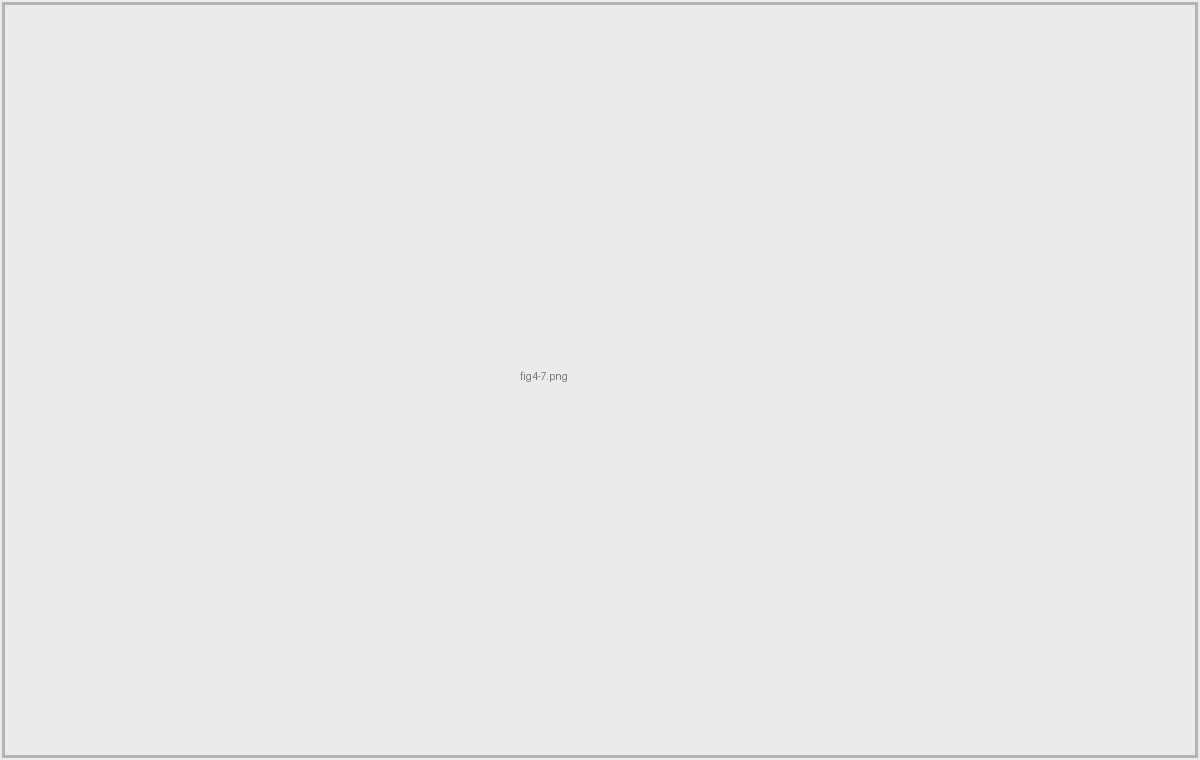
\includegraphics[width=\textwidth]{fig4-7.png}
    \caption{梯度波形与k空间轨迹：需求梯度波形（左，原图为红色实线）以最大梯度切换率线性增长直至达到最大梯度强度。图\autoref{fig:4.8}中的真实梯度系统对该梯度波形进行低通滤波（左，原图为绿色虚线），导致k空间轨迹发生畸变（右），在此尺度下几乎不可察觉。}
    \label{fig:4.7}
\end{figure}

\begin{figure}[ht]
    \centering
    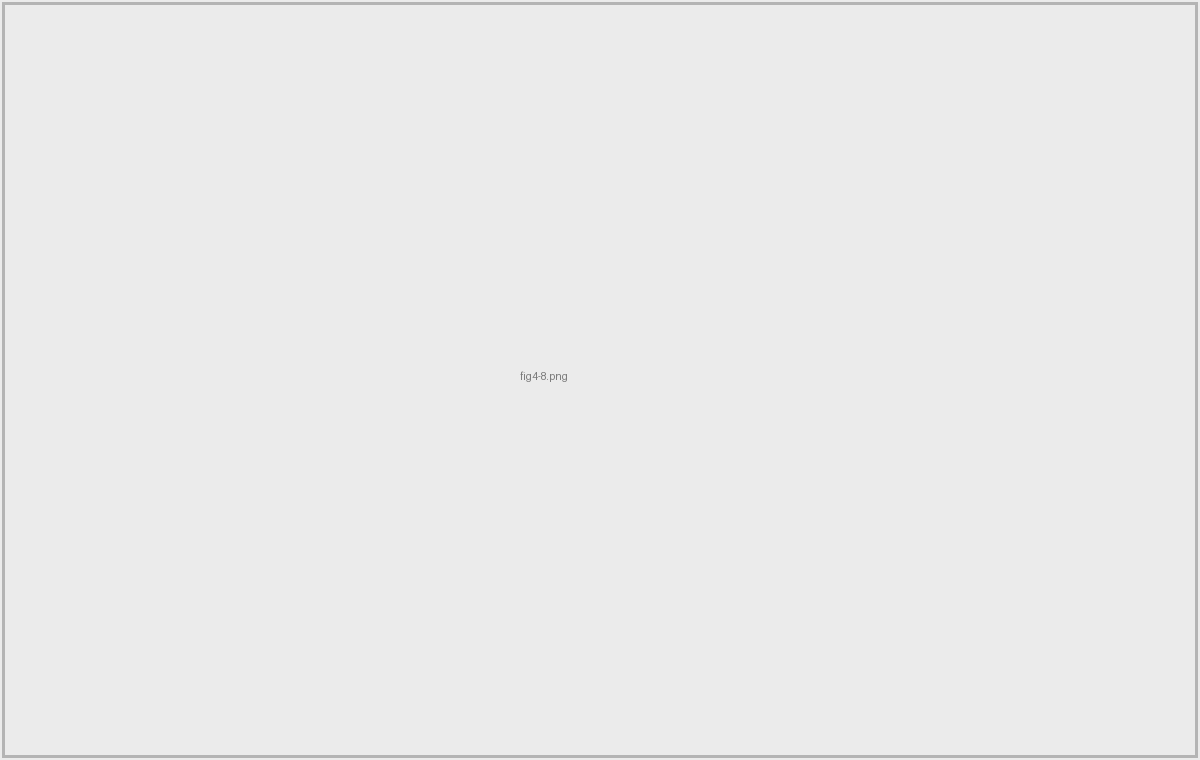
\includegraphics[width=\textwidth]{fig4-8.png}
    \caption{梯度系统表征：理想梯度系统（原图为红色实线）具有不变的幅度响应（左）与相位响应（右），而真实梯度系统（原图为绿色虚线）通常表现为随频率衰减的幅度响应与随频率增长的相位响应。}
    \label{fig:4.8}
\end{figure}

\begin{figure}[ht]
    \centering
    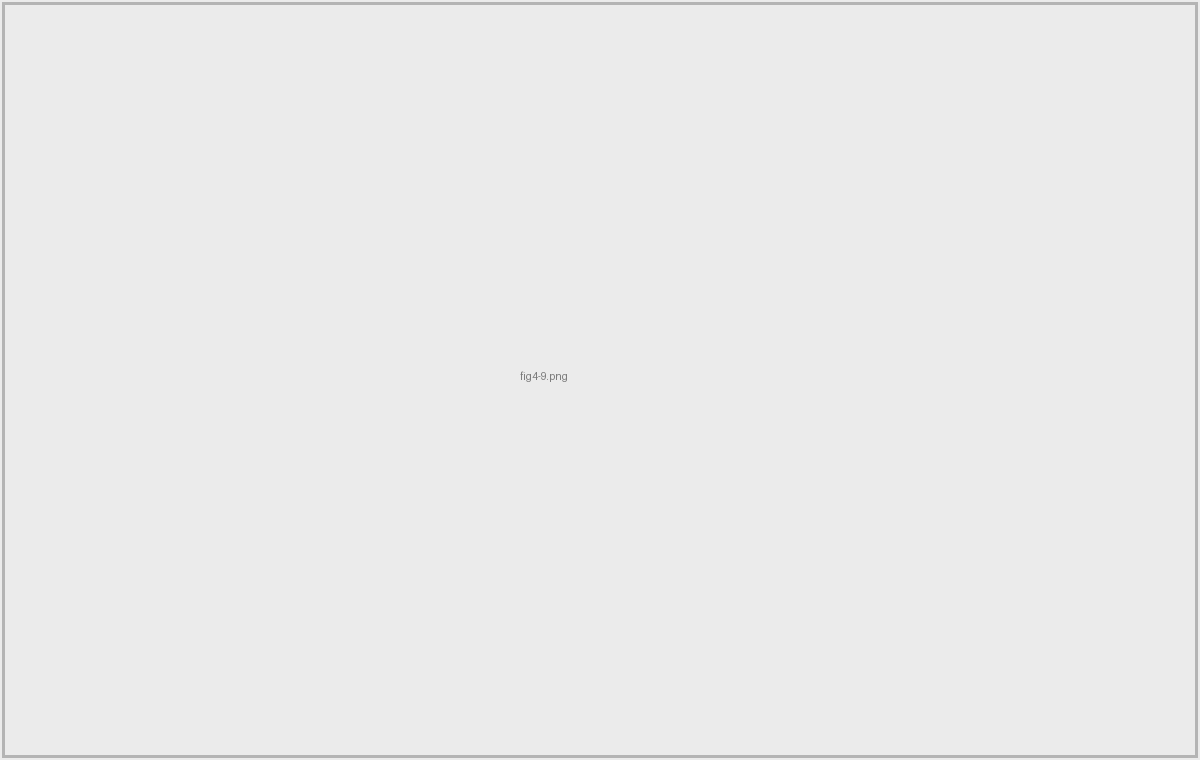
\includegraphics[width=\textwidth]{fig4-9.png}
    \caption{一维与二维采样模式：由图\autoref{fig:4.7}中的k空间轨迹，通过绕原点等角旋转生成一维（$k_x$）与二维（$k_x,k_y$）采样模式。与理想梯度系统（左）不同，使用更接近实际的梯度系统（右）得到的采样模式在k空间中心留下一个间隙，两幅图均对该间隙作了放大。}
    \label{fig:4.9}
\end{figure}

对$s$的非等距采样应用网格化，产生的误差绘制于图\autoref{fig:4.10}。使用理想梯度系统时观察到中等的偏移，而使用更接近实际的梯度系统时，明显的主要误差来自该间隙。

\begin{figure}[ht]
    \centering
    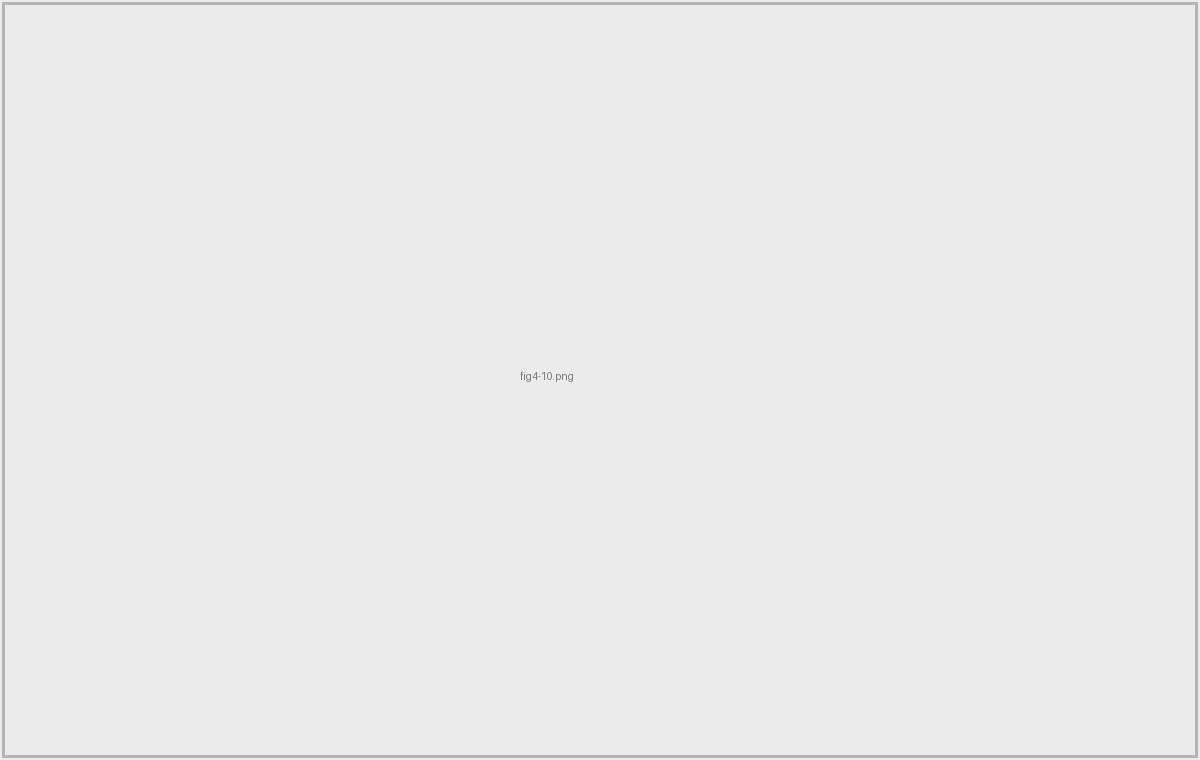
\includegraphics[width=\textwidth]{fig4-10.png}
    \caption{一维非笛卡尔采样：网格化。使用图\autoref{fig:4.9}中的两种非等距一维采样模式，以两倍空间分辨率用网格化重建一维物体$\hat{x}$。误差相对于连续三角形函数$x$计算。}
    \label{fig:4.10}
\end{figure}

到目前为止，所用的采样密度补偿基于相邻k空间采样位置之间的距离。对于更接近实际的梯度系统这一有问题情形，几何方法得到的权与上一节所述其他一些方法得到的权并列于图\autoref{fig:4.11}，连同相应的误差。按\autoref{equ:4.56}的不动点迭代从$\bm{w}^{[0]}=\frac{1}{N}\bm{1}$缓慢收敛，此时权始终保持为正。本例中采用了截断到两个旁瓣的$\operatorname{sinc}^2$卷积核，以把非等距样本直接映射到非等距样本。误差起初下降，但很快被因省略旁瓣而导致的权的系统性高估所主导。相比之下，强制$\|\bm{w}\|_1=1$可使误差整体降低两个数量级，但继续迭代时结果又会变差。求解\autoref{equ:4.55}与\autoref{equ:4.52}得到的权，对k空间中心的采样位置仍表现出显著而出人意料的振荡，但不再一定为正。第一种情形选用与之前相同的卷积核，第二种情形选用\autoref{equ:4.15}的Dirichlet核。不带显式正则化的CG方法只在第二种情形下可靠收敛，此时也获得了最低的误差。

\begin{figure}[ht]
    \centering
    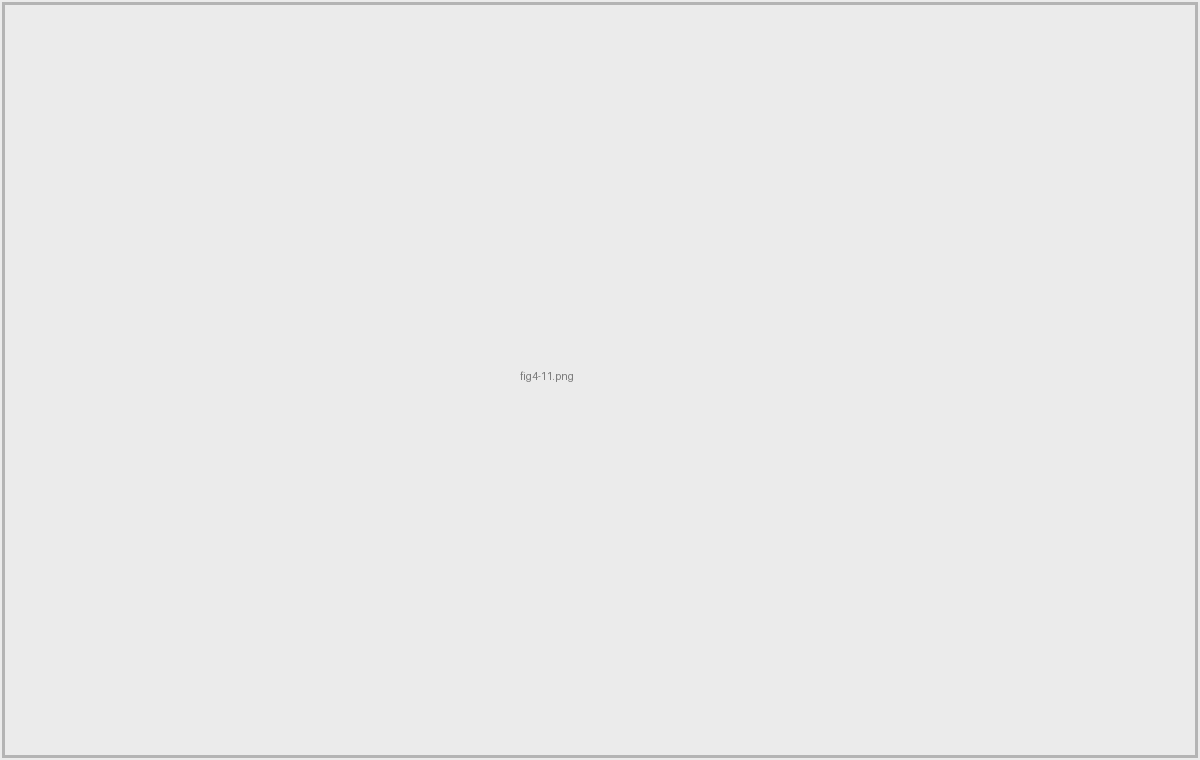
\includegraphics[width=\textwidth]{fig4-11.png}
    \caption{采样密度补偿：由图\autoref{fig:4.9}中第二种非等距一维采样模式导出采样密度补偿的权（左）：几何方法（上方原图为黑色）、基于重复网格化的数值方法，迭代次数分别为5（上方原图为红色）、25（上方原图为绿色）与125（下方原图为蓝色），各自又分为归一化（实线）与不归一化（虚线）两种；以及基于\autoref{equ:4.55}（下方原图为红色）与\autoref{equ:4.52}（下方原图为绿色）的代数方法。用网格化重建一维物体$\hat{x}$，误差相对于连续三角形函数$x$计算（右）。}
    \label{fig:4.11}
\end{figure}

最后，作为参照，迭代重建所得结果见图\autoref{fig:4.12}。以$\hat{\bm{x}}^{[0]}=\bm{0}$初始化的CG方法，在等距采样情形下、以及在非等距采样情形下配合有利的采样密度补偿时，产生的误差与网格化相似。迭代重建中使用了NFFT与伴随NFFT，但没有使用采样密度补偿或显式正则化。

\begin{figure}[ht]
    \centering
    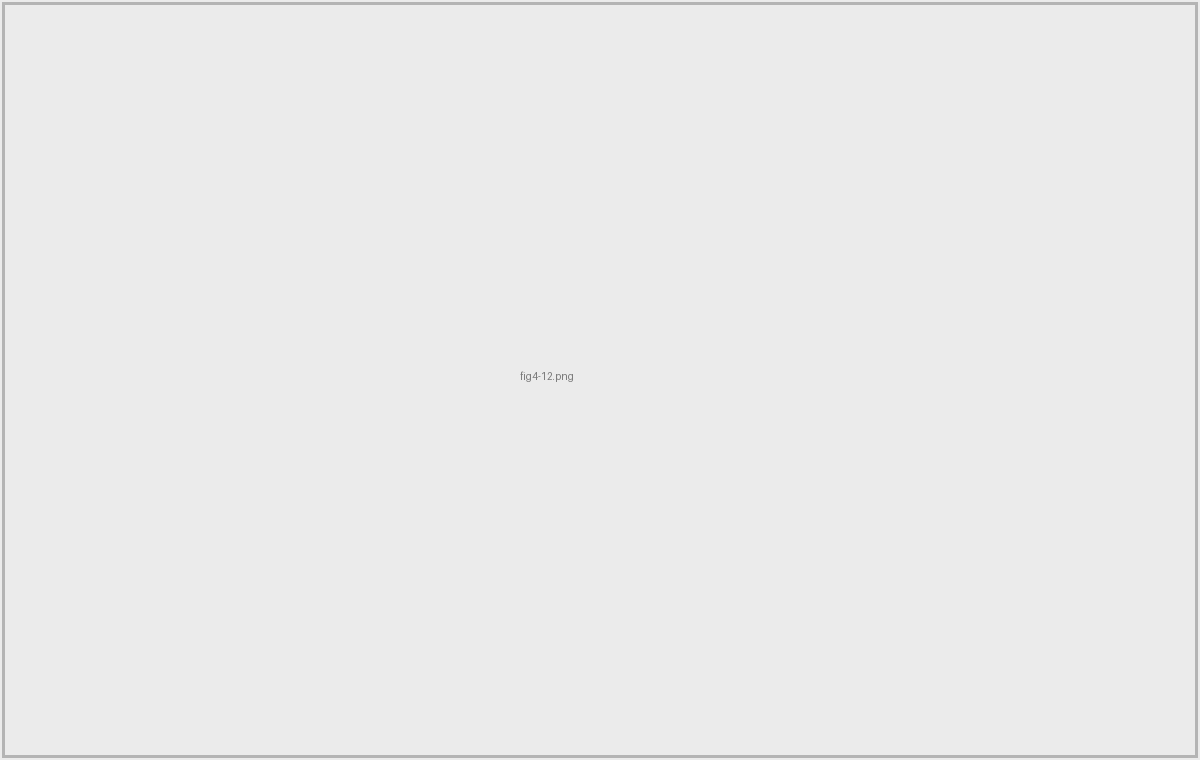
\includegraphics[width=\textwidth]{fig4-12.png}
    \caption{一维非笛卡尔采样：迭代重建。使用图\autoref{fig:4.9}中的两种非等距一维采样模式，以两倍空间分辨率迭代重建一维物体$\hat{x}$。误差相对于连续三角形函数$x$计算。}
    \label{fig:4.12}
\end{figure}

图\autoref{fig:4.13}所示的锥面函数被选作二维实例中的物体，以说明网格化。其Fourier变换由下式给出
\begin{equation}
    s(k_r)=\begin{cases}
        \dfrac{\pi^2\left(J_1(Rk_r)H_0(Rk_r)-J_0(Rk_r)H_1(Rk_r)\right)}{k_r^2}, & k_r\neq 0\\[3mm]
        \dfrac{1}{3}\pi R^2, & \text{其他}
    \end{cases},
    \label{equ:4.68}
\end{equation}
其中$J_0$、$J_1$与$H$分别表示第一类零阶、一阶Bessel函数与Struve函数\footnote{Struve函数$\mathbf{H}_\nu(x)$是Bessel方程的一个非齐次解，其定义与Bessel函数类似但带有额外的源项，常出现在具有圆形对称性的衍射与散射问题的解析解中。}。

\begin{figure}[ht]
    \centering
    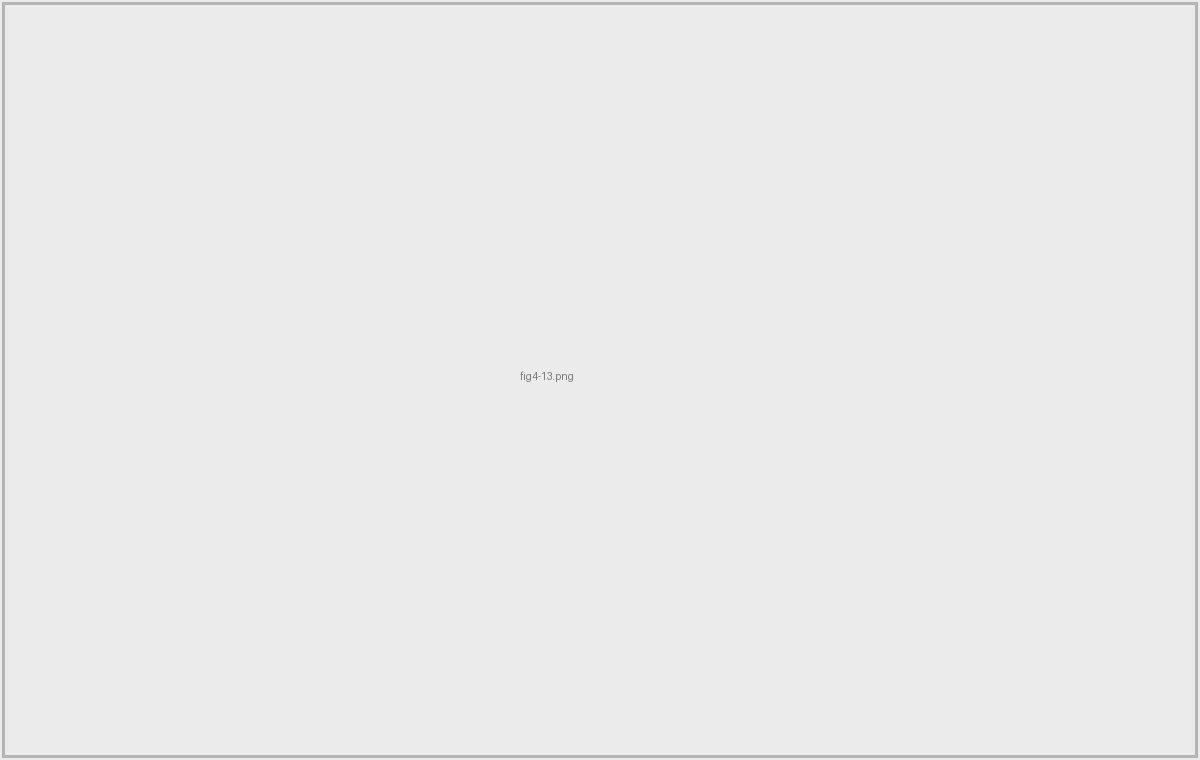
\includegraphics[width=\textwidth]{fig4-13.png}
    \caption{二维物体：选取一个连续锥面函数作为二维物体，其覆盖方形FOV的50\%、内切圆形FOV的64\%（左）。其频谱的幅度以对数刻度显示（右）。}
    \label{fig:4.13}
\end{figure}

对$s$的等距采样（$k_x$与$k_y\in[-\frac{1}{4},\frac{1}{4})$、$M=400^2$）分别应用逆FFT作为参照与网格化，所得误差绘制于图\autoref{fig:4.14}，主要由$r_x^2+r_y^2=320^2$处与原点处的振铃伪影主导——锥面函数在这两处不可微。网格化额外引入的误差仍然可忽略，尽管明显高于一维实例。此情形下网格化所需的浮点运算次数约为逆FFT的2.75倍，其中超过80\%由于过采样而花在Fourier变换上。

\begin{figure}[ht]
    \centering
    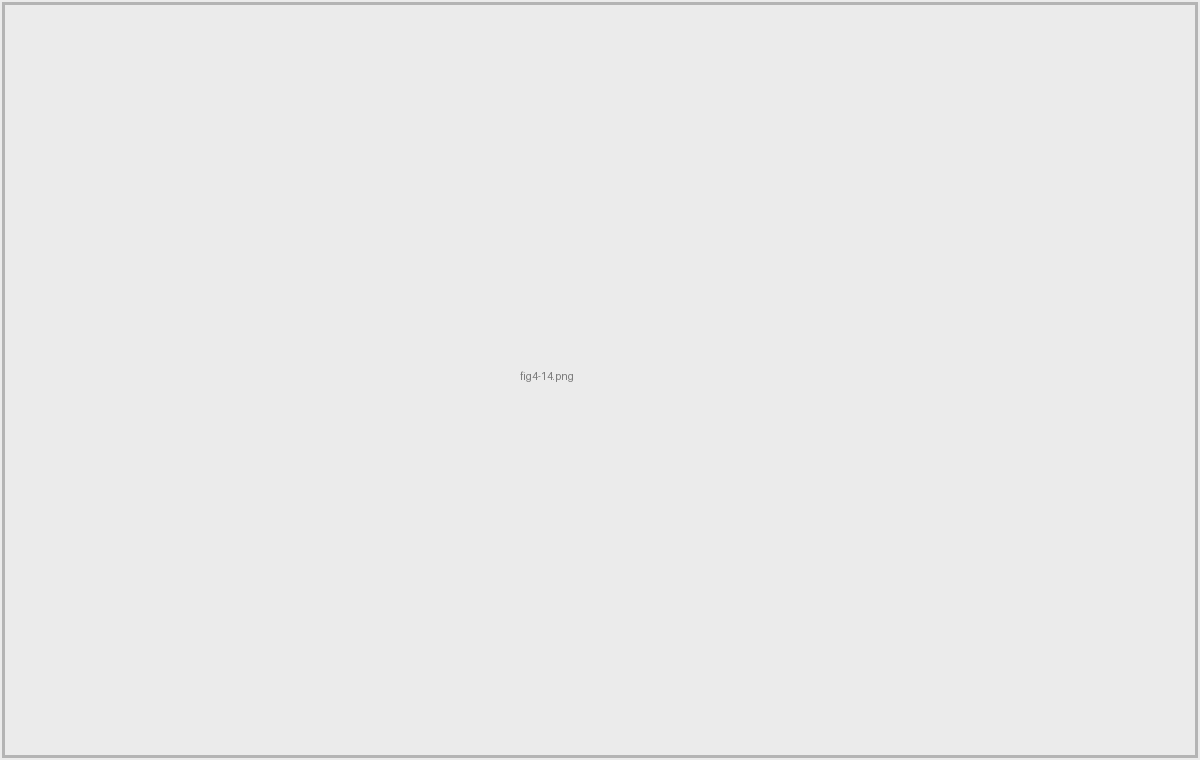
\includegraphics[width=\textwidth]{fig4-14.png}
    \caption{二维笛卡尔采样：逆FFT与网格化对比。由图\autoref{fig:4.13}中频谱的等距采样，以两倍空间分辨率重建二维物体，分别使用逆FFT（左）与网格化（右），均涉及补零。误差相对于连续锥面函数计算。}
    \label{fig:4.14}
\end{figure}

假设与一维实例相同的读出梯度来模拟$s$的非等距采样，但数据采集重复$\lceil\pi\sqrt{M}\rceil=1257$次。每次之后读出梯度的方向绕k空间原点旋转一个恒定角度，二维k空间中的采样位置也随之旋转。重复次数选取得使方位角方向上相邻采样位置之间的距离不超过$\frac{1}{2}\sqrt{M}$。这样就避免了欠采样。所得的采样模式覆盖一个圆形k空间区域，如图\autoref{fig:4.9}所示，其中方位角方向上看似连续的采样来自k空间中心的高采样密度。

对$s$的非等距采样分别应用网格化与迭代重建，所得误差绘制于图\autoref{fig:4.15}与图\autoref{fig:4.16}。采样密度补偿的权由几何方法导出，且只用于网格化。最值得注意的是，在更接近实际的梯度系统情形下，网格化所得误差相对一维实例降低了一个数量级。

\begin{figure}[ht]
    \centering
    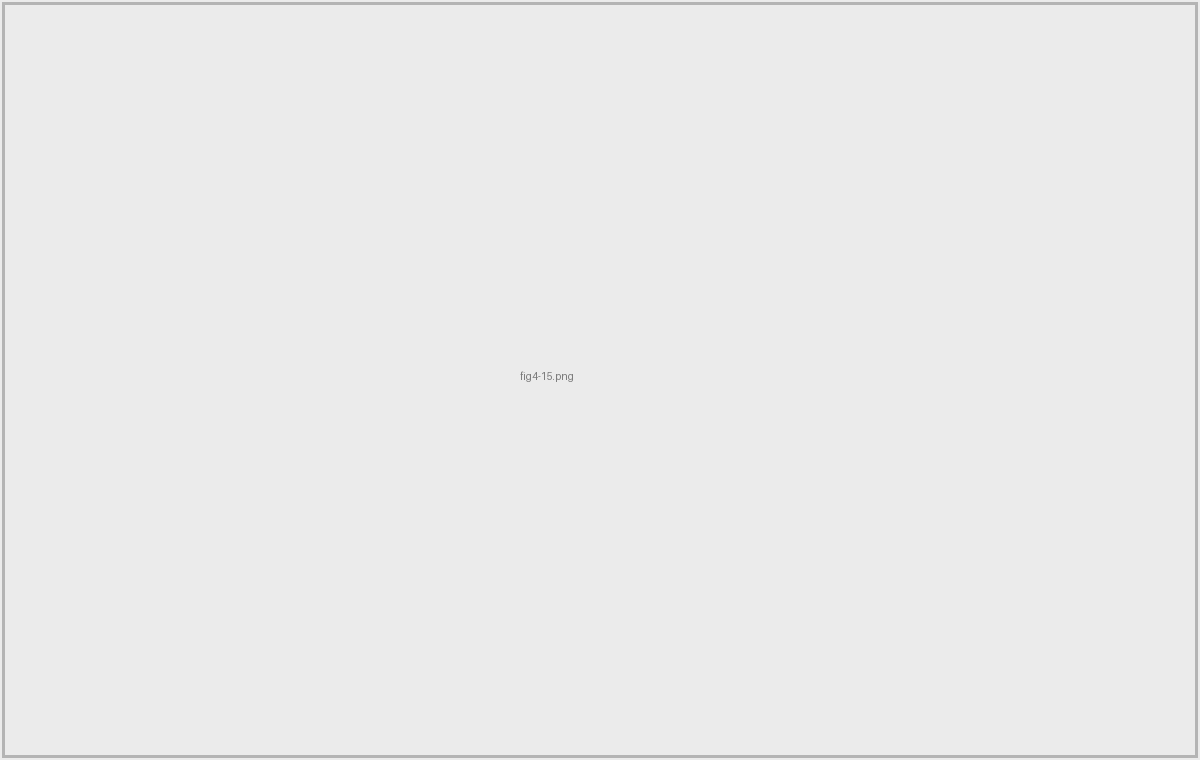
\includegraphics[width=\textwidth]{fig4-15.png}
    \caption{二维非笛卡尔采样：网格化。使用图\autoref{fig:4.9}中的两种非等距二维采样模式，以两倍空间分辨率用网格化重建二维物体。误差相对于连续锥面函数计算。}
    \label{fig:4.15}
\end{figure}

\begin{figure}[ht]
    \centering
    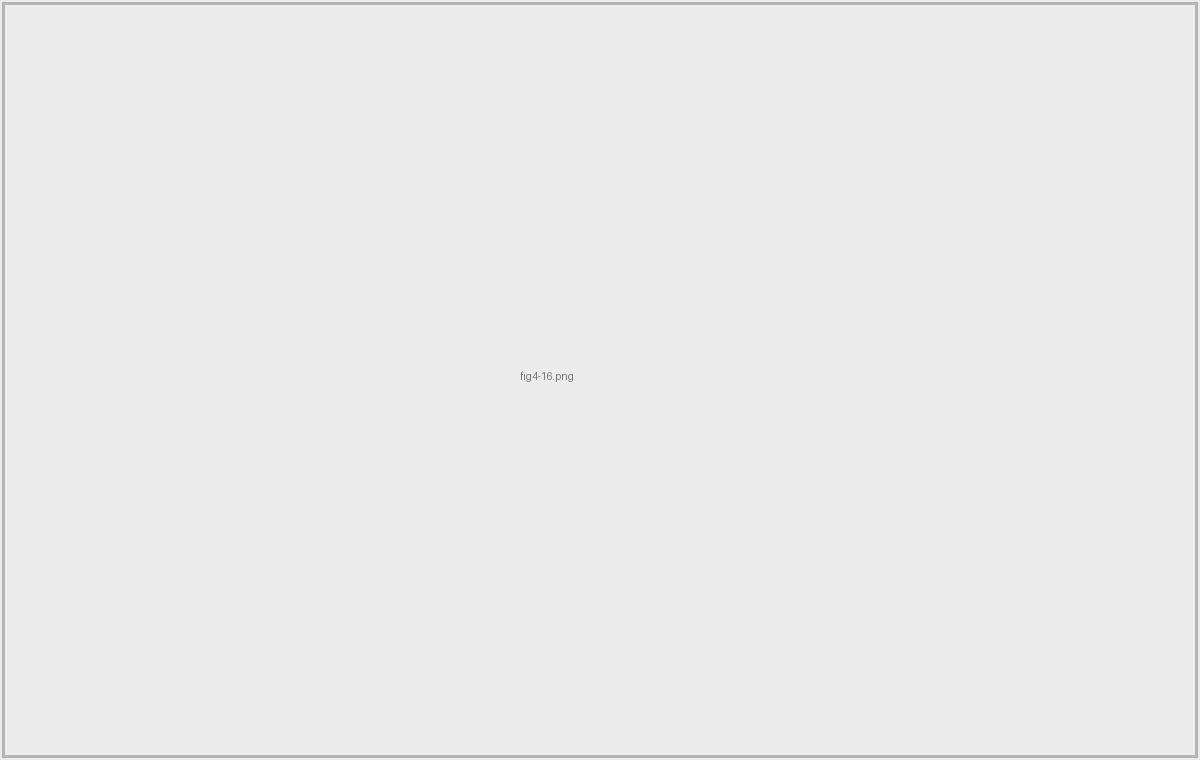
\includegraphics[width=\textwidth]{fig4-16.png}
    \caption{二维非笛卡尔采样：迭代重建。由图\autoref{fig:4.9}中的两种非等距二维采样模式，以两倍空间分辨率迭代重建二维物体。误差相对于连续锥面函数计算。}
    \label{fig:4.16}
\end{figure}

迭代重建的收敛性在图\autoref{fig:4.17}中分析。相比不使用采样密度补偿的\autoref{equ:4.59}，使用带采样密度补偿的\autoref{equ:4.61}会带来可观的加速，但在有噪声时对收敛有不利影响，这就要求要么施加合适的显式正则化，要么足够早地终止迭代。

\begin{figure}[ht]
    \centering
    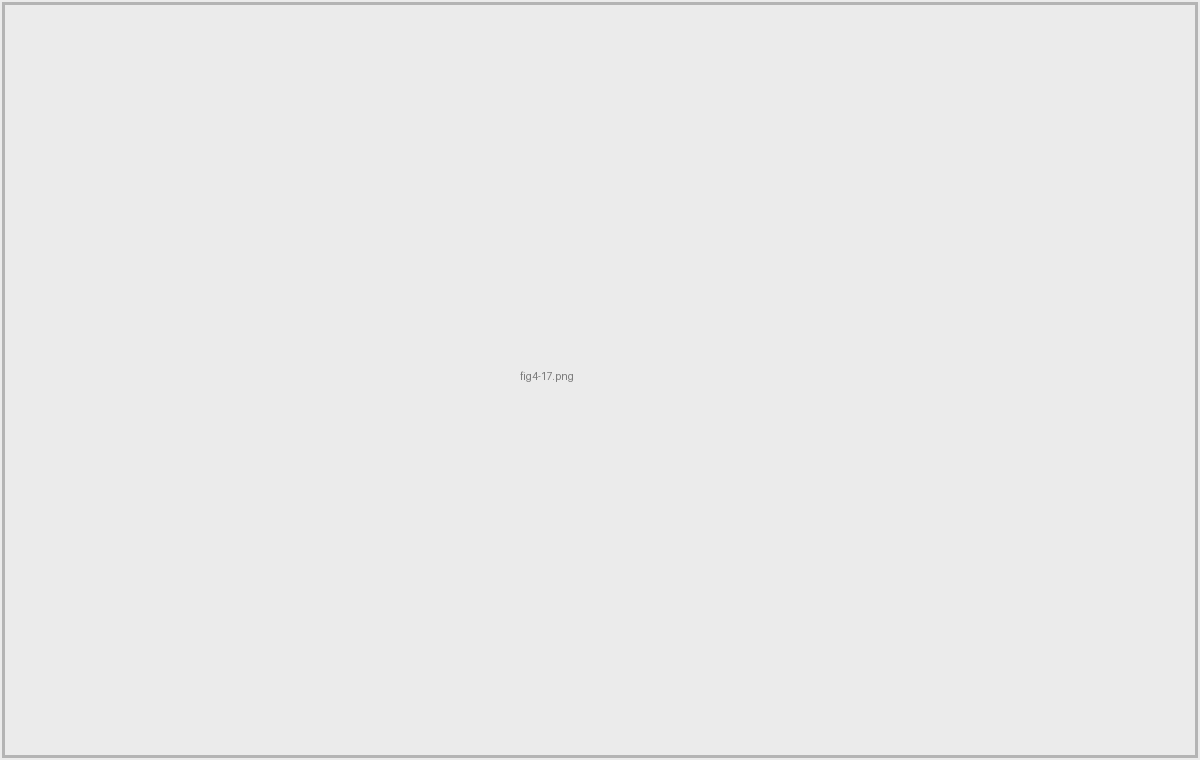
\includegraphics[width=\textwidth]{fig4-17.png}
    \caption{二维非笛卡尔采样：收敛性。二维物体分别在不使用（原图为红色实线）与使用（原图为绿色虚线）采样密度补偿的情况下迭代重建，又分别在不加噪（左）与加入标称SNR为50的噪声（右）的情况下重建。相对于连续锥面函数的均方误差作为迭代次数的函数绘制。}
    \label{fig:4.17}
\end{figure}

\section{空间分辨率与噪声}
尤其在把非笛卡尔成像与笛卡尔成像相比较时，意识到空间分辨率与噪声方面可能存在的差异至关重要，因此本节提出这一点。

空间分辨率的常用度量是PSF主瓣的半高全宽（Full Width at Half Maximum，FWHM）\label{term:FWHM}。在一维笛卡尔成像中，PSF由\autoref{equ:4.37}给出，并在$M=N$且$\frac{r}{N}$较小时近似为
\begin{equation}
    \operatorname{PSF}(r)\approx\operatorname{sinc}(\pi r).
    \label{equ:4.69}
\end{equation}
由于$\operatorname{sinc}(0.603\pi)=0.5$，FWHM等于$1.21$。在二维笛卡尔成像中，PSF沿$r_x$与$r_y$轴保持不变，但沿对角线$r_d$变为
\begin{equation}
    \operatorname{PSF}(r_d)\approx\operatorname{sinc}^2\left(\pi\sqrt{2}r_d\right),
    \label{equ:4.70}
\end{equation}
其中$r_d=\sqrt{2}r_x$且$r_y=\pm r_x$，假设采集覆盖方形k空间区域。FWHM增大到$1.25$，表明空间分辨率略有各向异性。

在二维非笛卡尔成像中，通常只覆盖较小的圆形k空间区域，如图\autoref{fig:4.1}所示。PSF近似为
\begin{equation}
    \operatorname{PSF}(r)\approx 2\operatorname{jinc}(\pi r),
    \label{equ:4.71}
\end{equation}
其中
\begin{equation}
    \operatorname{jinc}(x)=\begin{cases}
        \dfrac{J_1(x)}{x}, & x\neq 0\\[2mm]
        \dfrac{1}{2}, & \text{其他}
    \end{cases},
    \label{equ:4.72}
\end{equation}
FWHM为$1.41$，与方向无关。\autoref{equ:4.71}与\autoref{equ:4.69}、\autoref{equ:4.70}一样，可以通过假设对所覆盖的k空间区域进行连续采样来推导。

为使空间分辨率与二维笛卡尔成像相匹配，必须相对方形k空间区域扩大圆形k空间区域。把前者的半径缩放$\frac{2}{\sqrt{\pi}}=1.13$可使二者面积相等。应用于\autoref{equ:4.71}得到
\begin{equation}
    \operatorname{PSF}(r)\approx 2\operatorname{jinc}\left(2\sqrt{\pi}r\right)
    \label{equ:4.73}
\end{equation}
以及$1.25$的FWHM。这示于图\autoref{fig:4.18}，其中绘制了按\autoref{equ:4.69}、\autoref{equ:4.70}、\autoref{equ:4.71}与\autoref{equ:4.73}的PSF。值得注意的是，二维笛卡尔成像中沿轴的PSF第一旁瓣幅度最高。一般而言，这导致二维笛卡尔成像中的振铃伪影比二维非笛卡尔成像更明显。

\begin{figure}[ht]
    \centering
    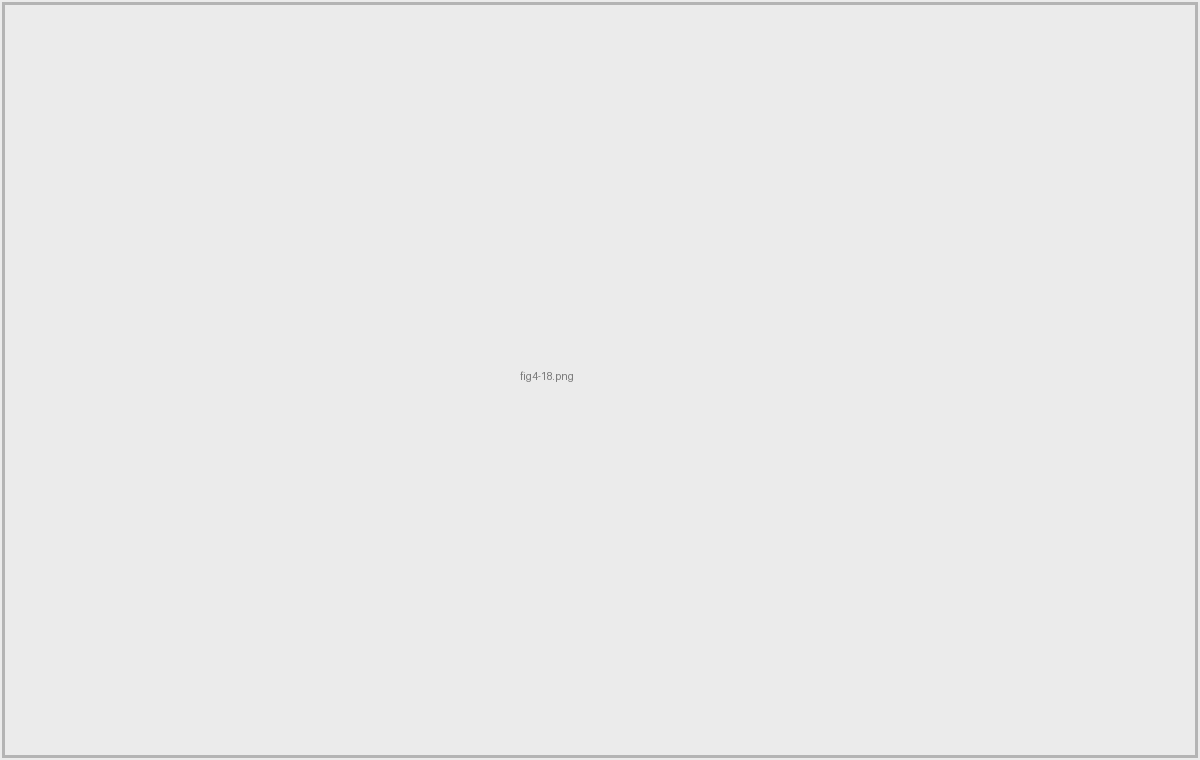
\includegraphics[width=\textwidth]{fig4-18.png}
    \caption{空间分辨率：对覆盖方形FOV的采集，沿轴（原图为红色实线）与沿对角线（原图为绿色实线）近似PSF；对圆形FOV，分别取方形内切圆（原图为蓝色实线）与面积相等的圆（原图为蓝色虚线）。图中标出了主瓣与半最大幅度水平线的交点。}
    \label{fig:4.18}
\end{figure}

连续采样近似的有效性在图\autoref{fig:4.19}中得到证实。尽管样本数相当少，使用带采样密度补偿的网格化对PROPELLER、径向与螺旋成像计算出的PSF彼此高度吻合，在此尺度下已无法分辨，并且与图\autoref{fig:4.18}中近似的PSF吻合。沿轴与沿对角线的EPI的计算PSF与近似PSF同样一致。自然，这仅对主瓣与前几个旁瓣成立。

\begin{figure}[ht]
    \centering
    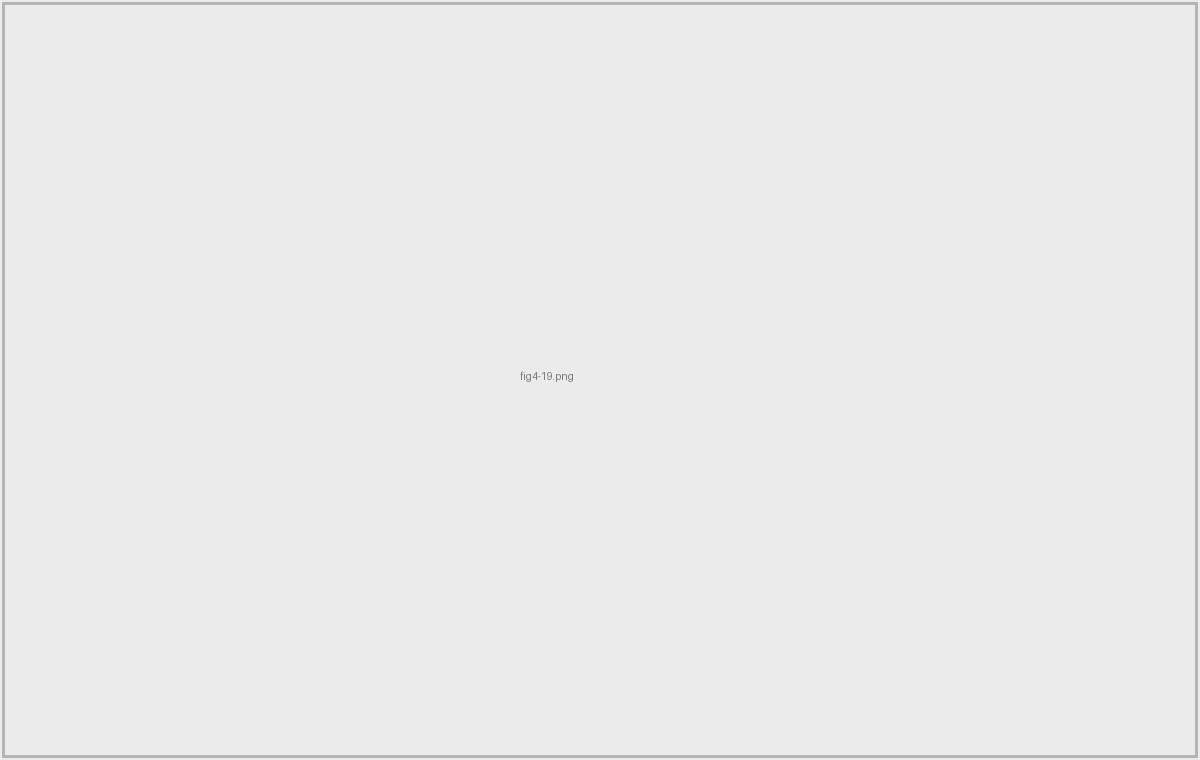
\includegraphics[width=\textwidth]{fig4-19.png}
    \caption{点扩散函数：对图\autoref{fig:4.1}中的采样模式计算PSF，即EPI沿轴（左，原图为红色）与沿对角线（左，原图为绿色），以及PROPELLER（右，原图为红色）、径向（右，原图为绿色）与螺旋（右，原图为蓝色）成像，网格化分别在不使用（虚线）与使用（实线）采样密度补偿的情况下进行。}
    \label{fig:4.19}
\end{figure}

尽管采样密度补偿对于用网格化塑造非笛卡尔成像的PSF至关重要，它会以如下因子降低SNR
\begin{equation}
    \frac{\sum_{m=1}^{M}[\bm{w}]_m}{\sqrt{M}\|\bm{w}\|_2},
    \label{equ:4.74}
\end{equation}
假设加性白Gaussian噪声。该因子只有在权均匀时才等于$1.0$。对图\autoref{fig:4.1}的二维采样模式，它在回波平面、PROPELLER、径向与螺旋成像情形下分别降至$0.98$、$0.85$、$0.87$与$0.96$。对图\autoref{fig:4.9}的二维采样模式，由于径向方向上额外的非等距采样，它进一步从$0.87$降至$0.80$。

在图\autoref{fig:4.17}右图中，使用不带采样密度补偿的迭代重建也观察到相同的SNR降低。标称SNR为50对应均方误差$4\times10^{-4}$，前提是最大信号归一化为$1.0$且其他误差可忽略。100次迭代后实际均方误差为$6.3\times10^{-4}$，这意味着噪声方差被放大$1.58$倍、SNR损失20\%。然而，CG方法在迭代过程中提供了一种逐渐减弱的固有正则化，这在使用带采样密度补偿的迭代重建时尤为明显。噪声方差的放大最终由矩阵
\begin{equation}
    \mathbf{X}=\left(\mathbf{E}^H\mathbf{E}\right)^{-1}
    \label{equ:4.75}
\end{equation}
或
\begin{equation}
    \mathbf{X}=\left(\mathbf{E}^H\mathbf{W}\mathbf{E}\right)^{-1}\left(\mathbf{E}^H\mathbf{W}^2\mathbf{E}\right)\left(\mathbf{E}^H\mathbf{W}\mathbf{E}\right)^{-1}
    \label{equ:4.76}
\end{equation}
的对角元给出；由于非笛卡尔成像中系统矩阵通常是病态的，若不施加显式正则化，它往往高得无法接受。

采样密度的变化还会导致有色噪声，其特征是功率谱密度非常数。有色噪声尤其会损害图像的感知空间分辨率。这可以通过添加噪声或在采样密度补偿中考虑其他准则（例如对比度）来缓解。

\section{扩展}
前面一节介绍了用于把空间中的等距样本高效转换为k空间中非等距样本的NFFT。此外还说明，伴随NFFT是网格化的组成部分，并与NFFT一起构成非笛卡尔成像迭代重建的组成部分。对于其他相关转换还存在别的NFFT，它们与笛卡尔成像和非笛卡尔成像都相关。本节概述它们及其应用。

为把空间中的非等距样本映射为k空间中的等距样本，与\autoref{equ:4.11}类似地得到近似
\begin{equation}
    \mathrm{e}^{-i2\pi kr}\approx\frac{1}{f\tilde{c}_{-Nk}}\sum_{n'=-fN/2}^{fN/2-1}\tilde{c}\left(r-\frac{n'}{f}\right)\mathrm{e}^{-i2\pi k\frac{n'}{f}},
    \label{equ:4.77}
\end{equation}
其中已考虑$r$与$k$的不同范围以及$\tilde{c}$必要的拉伸与缩放。它导出正演模型
\begin{equation}
    \tilde{s}_n\approx\frac{1}{f\tilde{c}_{-Nk_n}}\sum_{n'=-fN/2}^{fN/2-1}\left[\sum_{m=1}^{M}x_m\tilde{c}\left(r_m-\frac{n'}{f}\right)\right]\mathrm{e}^{-i2\pi k_n\frac{n'}{f}},
    \label{equ:4.78}
\end{equation}
其中$k_n=-\frac{1}{2},-\frac{1}{2}+\frac{1}{N},\ldots,\frac{1}{2}-\frac{1}{N}$。内层求和通过一次卷积把空间中的$M$个非等距样本转换为空间中$fN$个等距样本。外层求和相当于一次长度为$fN$的FFT，把空间中的等距样本变换为k空间中的等距样本。去变迹最后施加。

空间中的非等距样本出现在磁场梯度不理想（即空间上非常数）的情形，它影响空间编码，若在重建中忽略会导致图像失真。在这种情况下，k空间中测得的信号建模为
\begin{equation}
    s(\bm{k})=\int_{-N/2}^{N/2}x(\bm{r})\,\mathrm{e}^{-i2\pi\bm{k}g(\bm{r})}\,\mathrm{d}\bm{r},
    \label{equ:4.79}
\end{equation}
其中$g$通常是非线性函数，把真实位置$\bm{r}$映射到空间中的表观位置$\bm{r}'$。只要$g$可逆，变量替换给出
\begin{equation}
    s(\bm{k})=\int_{g(-N/2)}^{g(N/2)}x\left(g^{-1}(\bm{r}')\right)\frac{\mathrm{d}g^{-1}(\bm{r}')}{\mathrm{d}\bm{r}'}\mathrm{e}^{-i2\pi\bm{k}\bm{r}'}\,\mathrm{d}\bm{r}'
    \label{equ:4.80}
\end{equation}
以及$x$在非等距样本上的空间离散化。目前，畸变校正通常在空间重建之后、使用插值与缩放常规执行。然而，把它整合进重建有望带来优势，尤其在空间分辨率方面。这要求在笛卡尔成像中高效求值\autoref{equ:4.78}，而在非笛卡尔成像中正演模型必须推广到两个域都是非等距样本的情形。

空间中的非等距样本也由不理想的主磁场引起。此时信号描述为
\begin{equation}
    s(t)=\int_{-N/2}^{N/2}x(\bm{r})\,\mathrm{e}^{-i2\pi\bm{k}(t)\bm{r}}\mathrm{e}^{-i2\pi tf(\bm{r})}\,\mathrm{d}\bm{r},
    \label{equ:4.81}
\end{equation}
这里$s$与$\bm{k}$是$t$（激励后的时间）的显函数，$f$表示由主磁场空间变化引起的核自旋进动频率偏移。在笛卡尔成像中，由于读出梯度在数据采集期间保持不变，$\bm{k}$是线性函数。此时\autoref{equ:4.81}可写成\autoref{equ:4.79}。在EPI中，这一点在相位编码方向上仍然成立，而主要的畸变正出现在该方向。

非笛卡尔成像中主磁场不均匀性的考虑将在第十二章处理。这里只推导用于在两个域的非等距样本之间高效转换的NFFT，它已被证明可应用于此类偏共振校正。窗函数$c$的逆Fourier变换
\begin{equation}
    \left(\mathcal{F}^{-1}c\right)(r)=\int_{-\infty}^{\infty}c(k)\,\mathrm{e}^{i2\pi kr}\,\mathrm{d}k
    \label{equ:4.82}
\end{equation}
改写为
\begin{equation}
    \left(\mathcal{F}^{-1}c\right)(r)=\int_{-1/2}^{1/2}\sum_{p=-\infty}^{\infty}c(k+p)\,\mathrm{e}^{i2\pi(k+p)r}\,\mathrm{d}k
    \label{equ:4.83}
\end{equation}
并近似为
\begin{equation}
    \left(\mathcal{F}^{-1}c\right)(r)\approx\frac{1}{fN}\sum_{n'=-fN/2}^{fN/2-1}\sum_{p=-\infty}^{\infty}c\left(k-\frac{n'}{fN}+p\right)\mathrm{e}^{i2\pi\left(k-\frac{n'}{fN}+p\right)r}
    \label{equ:4.84}
\end{equation}
从而得到
\begin{equation}
    \mathrm{e}^{-i2\pi kr}\approx\frac{1}{fN\left(\mathcal{F}^{-1}c\right)(r)}\sum_{n'=-fN/2}^{fN/2-1}\sum_{p=-\infty}^{\infty}c\left(k-\frac{n'}{fN}+p\right)\mathrm{e}^{-i2\pi\left(\frac{n'}{fN}-p\right)r}.
    \label{equ:4.85}
\end{equation}
随后通过例如简单地把$c$的范围限制到$[-\frac{K}{2fN},\frac{K}{2fN}]$、把$k$的范围限制到$[-\frac{1}{2}+\frac{K}{2fN},\frac{1}{2}-\frac{K}{2fN})$，内层求和被消去，得到
\begin{equation}
    \mathrm{e}^{-i2\pi kr}\approx\frac{1}{fN\left(\mathcal{F}^{-1}c\right)(r)}\sum_{n'=-fN/2}^{fN/2-1}c'\left(k-\frac{n'}{fN}\right)\mathrm{e}^{-i2\pi\frac{n'}{fN}r}.
    \label{equ:4.86}
\end{equation}

这样的NFFT还允许在重建中纳入更高阶的磁场扰动，它们可以建模为
\begin{equation}
    s(t)=\int_{-N/2}^{N/2}x(\bm{r})\,\mathrm{e}^{-i2\pi\sum_{l=1}^{L}k_l(t)b_l(\bm{r})}\,\mathrm{d}\bm{r},
    \label{equ:4.87}
\end{equation}
其中$b$是空间基函数、$\bm{k}$是相应的时间变化系数。$b$通常选取球谐函数，而确定$\bm{k}$通常需要单独的校准测量（如梯度脉冲响应测量）或同步磁场监测。一阶球谐函数等价于空间常数磁场梯度，因而描述k空间中的实际采样位置。相应时间变化系数的准确知识通常是必要的，但也足以在非笛卡尔成像中获得足够的图像质量。

最后，数据采集期间的指数信号衰减可以通过向$f$加上适当缩放的衰减率作为虚部而纳入\autoref{equ:4.81}。

\section{小结}
NFFT是非笛卡尔MRI重建不可或缺的组成部分。它们把FFT推广到非等距样本，并依赖一种精度可控的近似——即便在很小的过采样因子与核尺寸下，对MRI而言也已足够。如今已有若干优化实现可用于各种计算平台，也以其他缩写出现，如NUFFT与FINUFFT。它们大大便利了应对各种采样模式的通用算法的开发与应用，也进一步缓解了人们对NFFT运行时间的担忧。

本章描述了两种这样的算法：网格化与迭代重建。网格化除了一次伴随NFFT之外还涉及采样密度补偿，借此对大多数流行的采样模式都能达到合理的精度。迭代重建同时包含NFFT与伴随NFFT，可以以计算复杂度为代价获得更好的精度。这两种算法构成了后续各章所讨论的其他算法的基础，后者尤其通过欠采样支持非笛卡尔成像的加速。

NFFT还被证明是对不理想主磁场与磁场梯度进行校正的有价值的组成部分。使这些校正更加稳健——尤其是在没有干扰参数准确知识的情况下——仍然是一个相当大的挑战。

尽管迄今为止已提出并研究了许多非笛卡尔成像方法，但目前只有少数在更大范围上被临床常规采用。非笛卡尔成像方法的使用是否会进一步扩大、甚至与笛卡尔成像方法的使用相抗衡，仍有待观察。

\newpage
\appendix
\section{物理量符号及含义}
\begin{table}[h]
    \small
    \centering
    \begin{tabularx}{\textwidth}{c X c}
        \toprule
        \textbf{符号} & \textbf{含义} & \textbf{单位/类型} \\
        \midrule
        $\gamma$ & 旋磁比 & $\mathrm{rad}\,\mathrm{s}^{-1}\mathrm{T}^{-1}$ \\
        $\bm{G}$ & 磁场梯度（梯度波形） & $\mathrm{T}/\mathrm{m}$ \\
        $\bm{k}$ & k空间采样位置 & $\mathrm{m}^{-1}$ \\
        $t$ & 时间（激励后） & $\mathrm{s}$ \\
        $s$ & k空间信号 & $\mathbb{C}$ \\
        $x$ & 物体的横向磁化强度（待重建图像） & $\mathbb{C}$ \\
        $N$ & FOV内的采样点数／图像像素数 & $\mathbb{N}$ \\
        $\bm{r}$ & 空间坐标 & $\mathrm{m}$ \\
        $M$ & k空间样本总数 & $\mathbb{N}$ \\
        $f$ & 过采样因子（$f\ge 1$） & 无量纲 \\
        $c$ & 窗函数 & --- \\
        $\tilde{c}$ & 周期为1的周期化窗函数 & --- \\
        $\tilde{c}_r$ & 窗函数的Fourier系数（去变迹） & --- \\
        $K$ & 卷积核尺寸 & $\mathbb{N}$ \\
        $b$ & Kaiser--Bessel窗的形状参数 & --- \\
        $I_0$ & 第一类零阶修正Bessel函数 & --- \\
        $\mathbf{D}$ & $N\times N$对角去变迹矩阵 & --- \\
        $\mathbf{F}$ & $fN\times N$ Fourier变换矩阵 & --- \\
        $\mathbf{C}',\mathbf{C}$ & $M\times fN$卷积矩阵（稀疏／稠密） & --- \\
        $\mathbf{E}$ & $M\times N$编码矩阵 & --- \\
        $\hat{\bm{x}}$ & 重建图像估计 & $\mathbb{C}^N$ \\
        $\operatorname{PSF}$ & 点扩散函数 & --- \\
        $\mathbf{W}$ & 由权向量构成的对角矩阵 & --- \\
        $\bm{w}$ & 采样密度补偿的权向量 & $\mathbb{R}^M$ \\
        \bottomrule
    \end{tabularx}
\end{table}
\begin{table}[h]
    \small
    \centering
    \begin{tabularx}{\textwidth}{c X c}
        \toprule
        \textbf{符号} & \textbf{含义} & \textbf{单位/类型} \\
        \midrule
        $k_r,k_\phi$ & 极坐标下的径向与方位角方向 & 无量纲 \\
        $k_s,k_i$ & 螺旋轨迹中沿交错线与交错线编号的参数 & 无量纲 \\
        $\alpha$ & Archimedes螺线的参数（$\alpha\in[0,1]$） & 无量纲 \\
        $M_I,M_S$ & 交错线条数与每条交错线的样本数 & $\mathbb{N}$ \\
        $\mathbf{J}_R,\mathbf{J}_S$ & 径向／螺旋坐标变换的Jacobi矩阵 & --- \\
        $\mathbf{A},\bm{b}$ & 权的最小二乘线性系统矩阵与右端项 & --- \\
        $q$ & 系统矩阵元素构成的卷积核 & --- \\
        $R$ & 一维实例中三角形函数的半宽（$R=320$） & 无量纲 \\
        $H(i\omega)$ & 梯度系统的频率响应 & --- \\
        $T$ & 梯度系统的时间常数 & $\mathrm{s}$ \\
        $J_0,J_1$ & 第一类零阶、一阶Bessel函数 & --- \\
        $H$ & Struve函数 & --- \\
        $r_d$ & 二维Fourier空间的对角线坐标（$r_d=\sqrt{2}r_x$） & 无量纲 \\
        $\operatorname{jinc}$ & 一阶Bessel函数比定义的径向函数 & --- \\
        $\mathbf{X}$ & 噪声方差放大矩阵 & --- \\
        $g(\bm{r})$ & 梯度畸变的非线性坐标映射 & --- \\
        $f(\bm{r})$ & 主磁场不均匀引起的频率偏移 & $\mathrm{Hz}$ \\
        $b_l,\bm{k}_l$ & 磁场扰动的空间基函数与时间变化系数 & --- \\
        $L$ & 磁场扰动展开的阶数 & $\mathbb{N}$ \\
        \bottomrule
    \end{tabularx}
\end{table}

\newpage
\section{术语中英文及缩写索引}
下表按术语在正文中首次出现的先后顺序排列，页码为其首次出现位置。
\begin{table}[h]
    \small
    \centering
    \begin{tabularx}{\textwidth}{l X c r}
        \toprule
        \textbf{中文术语} & \textbf{英文全称} & \textbf{缩写} & \textbf{页码} \\
        \midrule
        计算机断层成像 & Computed Tomography & CT & \pageref{term:CT} \\
        快速Fourier变换 & Fast Fourier Transform & FFT & \pageref{term:FFT} \\
        回波平面成像 & Echo-Planar Imaging & EPI & \pageref{term:EPI} \\
        扩散加权成像 & Diffusion-Weighted Imaging & DWI & \pageref{term:DWI} \\
        功能磁共振成像 & functional MRI & fMRI & \pageref{term:fMRI} \\
        周期性旋转重叠平行线增强重建 & Periodically Rotated Overlapping Parallel Lines with Enhanced Reconstruction & PROPELLER & \pageref{term:PROPELLER} \\
        信噪比 & Signal-to-Noise Ratio & SNR & \pageref{term:SNR} \\
        非均匀快速Fourier变换 & Nonequispaced Fast Fourier Transform & NFFT & \pageref{term:NFFT} \\
        视野 & Field of View & FOV & \pageref{term:FOV} \\
        点扩散函数 & Point Spread Function & PSF & \pageref{term:PSF} \\
        共轭梯度 & Conjugate Gradient & CG & \pageref{term:CG} \\
        半高全宽 & Full Width at Half Maximum & FWHM & \pageref{term:FWHM} \\
        \bottomrule
    \end{tabularx}
\end{table}

\end{document}

\end{document}
